\documentclass{beamer}
\usetheme{Berkeley}
\usecolortheme{default}
%Formatting Packages
\usepackage{graphicx}
\usepackage{float}
\usepackage[final]{pdfpages}
\usepackage[yyyymmdd]{datetime}
\renewcommand{\dateseparator}{--}
\usepackage{textcomp}
\usepackage{paracol}
\usepackage[authoryear, sort]{natbib}

%Science packages
\usepackage{siunitx}
\usepackage{graphicx}
\usepackage[colorinlistoftodos]{todonotes}
\input macros.tex


%\usepackage[colorlinks=true, allcolors=blue]{hyperref}

%Document Details
\title{Methods to Detect Habitable Atmospheres on the Terrestrial Exoplanet
       TRAPPIST-1e}
\author{Dylan Gatlin}
\newdate{defense}{03}{04}{2019}
\date{\displaydate{defense}}

\begin{document}
\input .backend.tex

\begin{frame}
    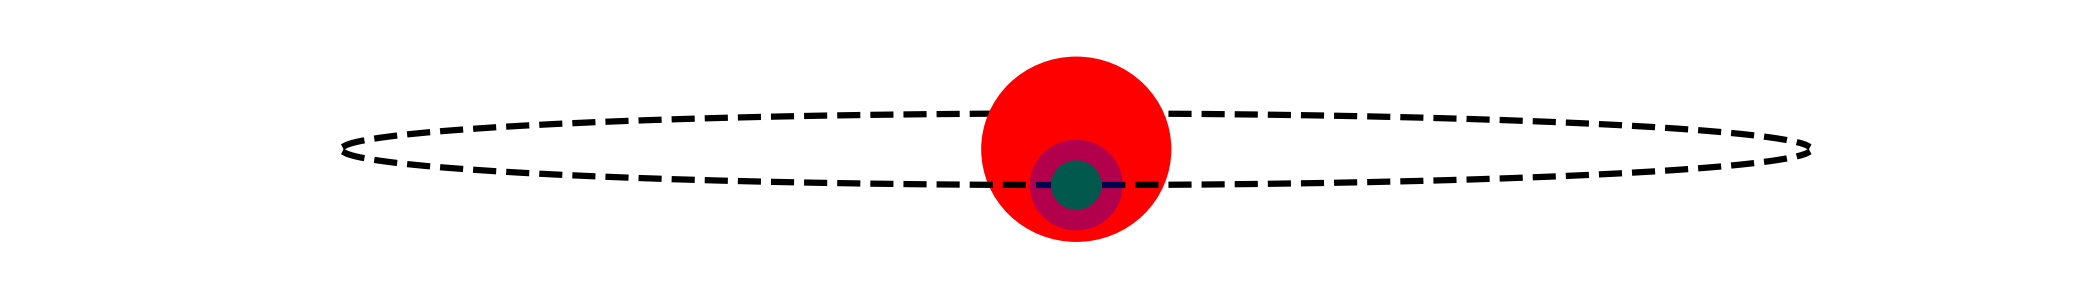
\includegraphics[width=\textwidth]{transit.png}
    \titlepage
\end{frame}

\begin{frame}
    \frametitle{Outline}
    \tableofcontents
\end{frame}

\section{Models}
\subsection{All models}
\begin{frame}
    \frametitle{TRAPPIST-1 e is the most likely candidate for life, but not all
    models are habitable}
    \begin{columns}
    \column{0.4\textwidth}
        \begin{table}
            \begin{tabular}{r|l}
                Orbital Period & 6.09d\\
                Radius & $0.95\mathrm{R}_\oplus$\\
                Mass & $0.77\mathrm{M}_\oplus$\\
                Surface gravity & $0.93\mathrm{g}_\oplus$\\
                Solar irradiance & $0.6\mathrm{S}_\oplus$\\
                $\mathrm{T}_*$ & $2511\mathrm{K}$\\
                Distance & 12.14pc\\
            \end{tabular}
            \caption{{\scriptsize Values provided by \citet{trappistdiscovery}}}
        \end{table}
    \column{0.6\textwidth}
        \begin{figure}
            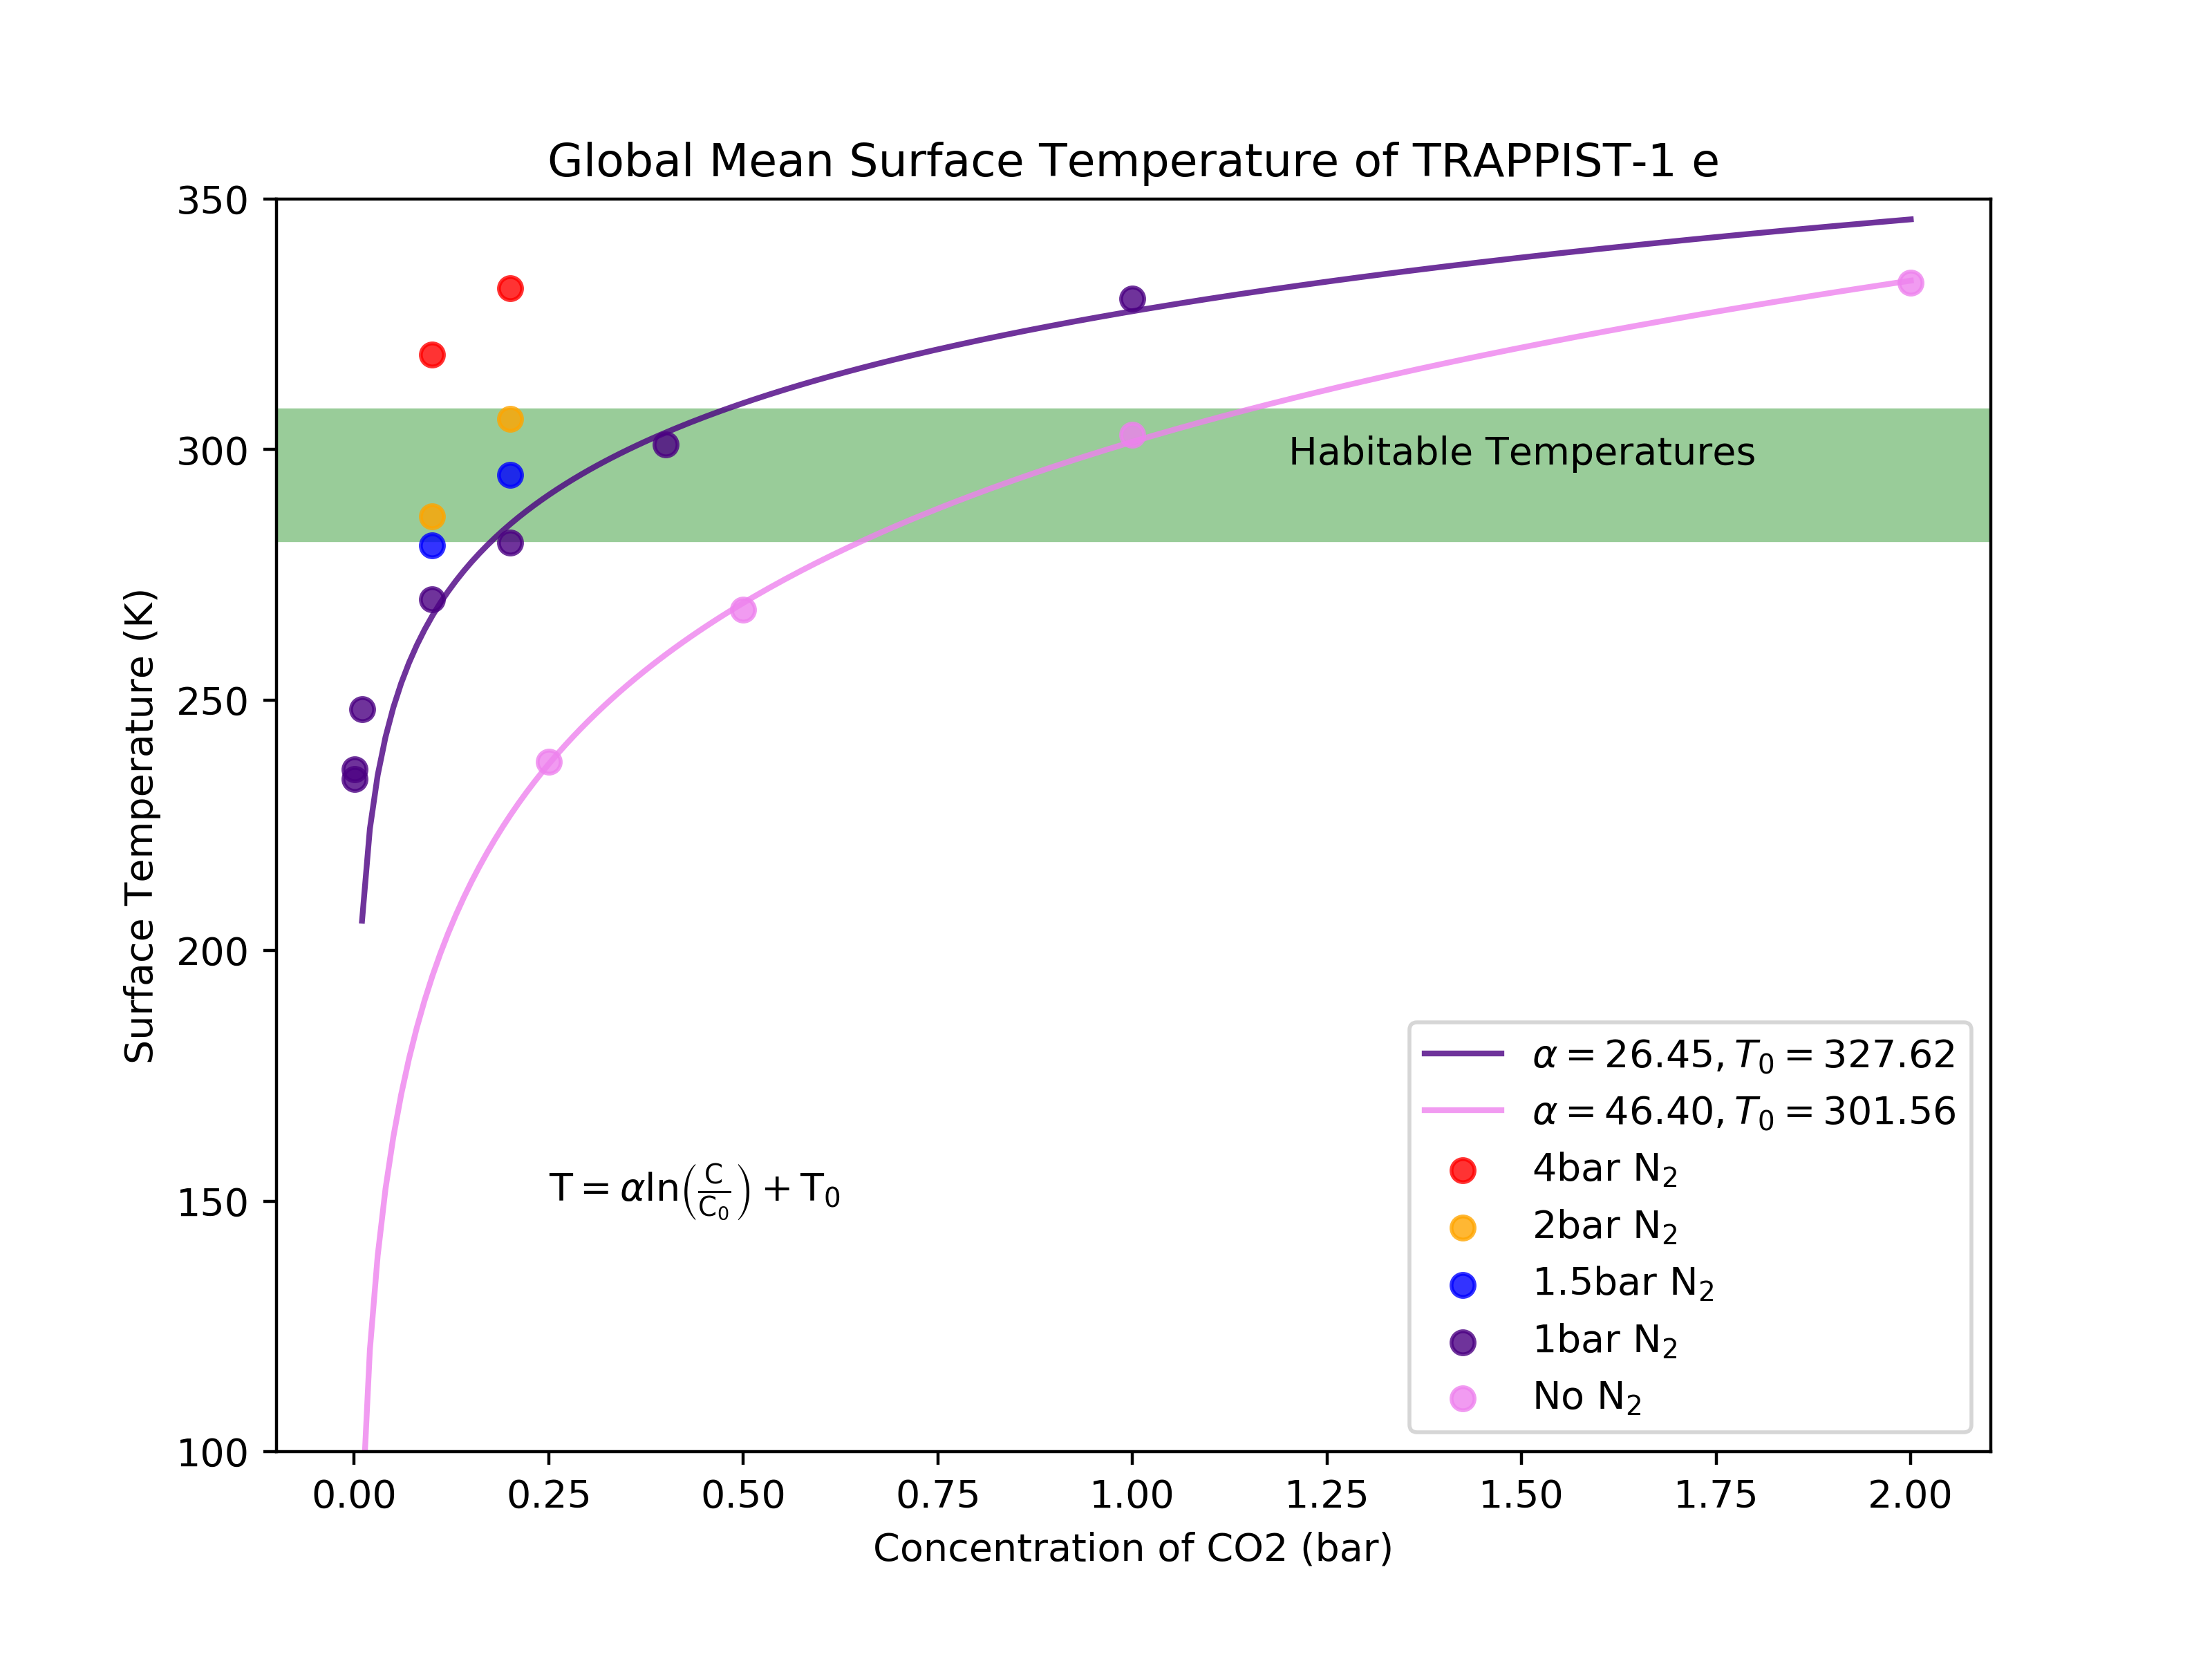
\includegraphics[width=\textwidth]{models/surfacet_co2.png}
            \caption{{\scriptsize Models provided by \citet{wolf17} and \citet{ravihabitablemoist}}}
        \end{figure}
    \end{columns}
\end{frame}

\subsection{Surface maps}

\begin{frame}
    \frametitle{TRAPPIST-1 e models have persistent clouds with unique
    structures}
    % \setlength{\topsep{0pt}}
    \begin{columns}
    \column{0.5\textwidth}
        {\tiny 1bar\chem{N_2} 0.4bar\chem{CO_2}}
    %     \vpsace{-6EM}
        \begin{figure}[topsep=0pt, partopsep=0pt]
        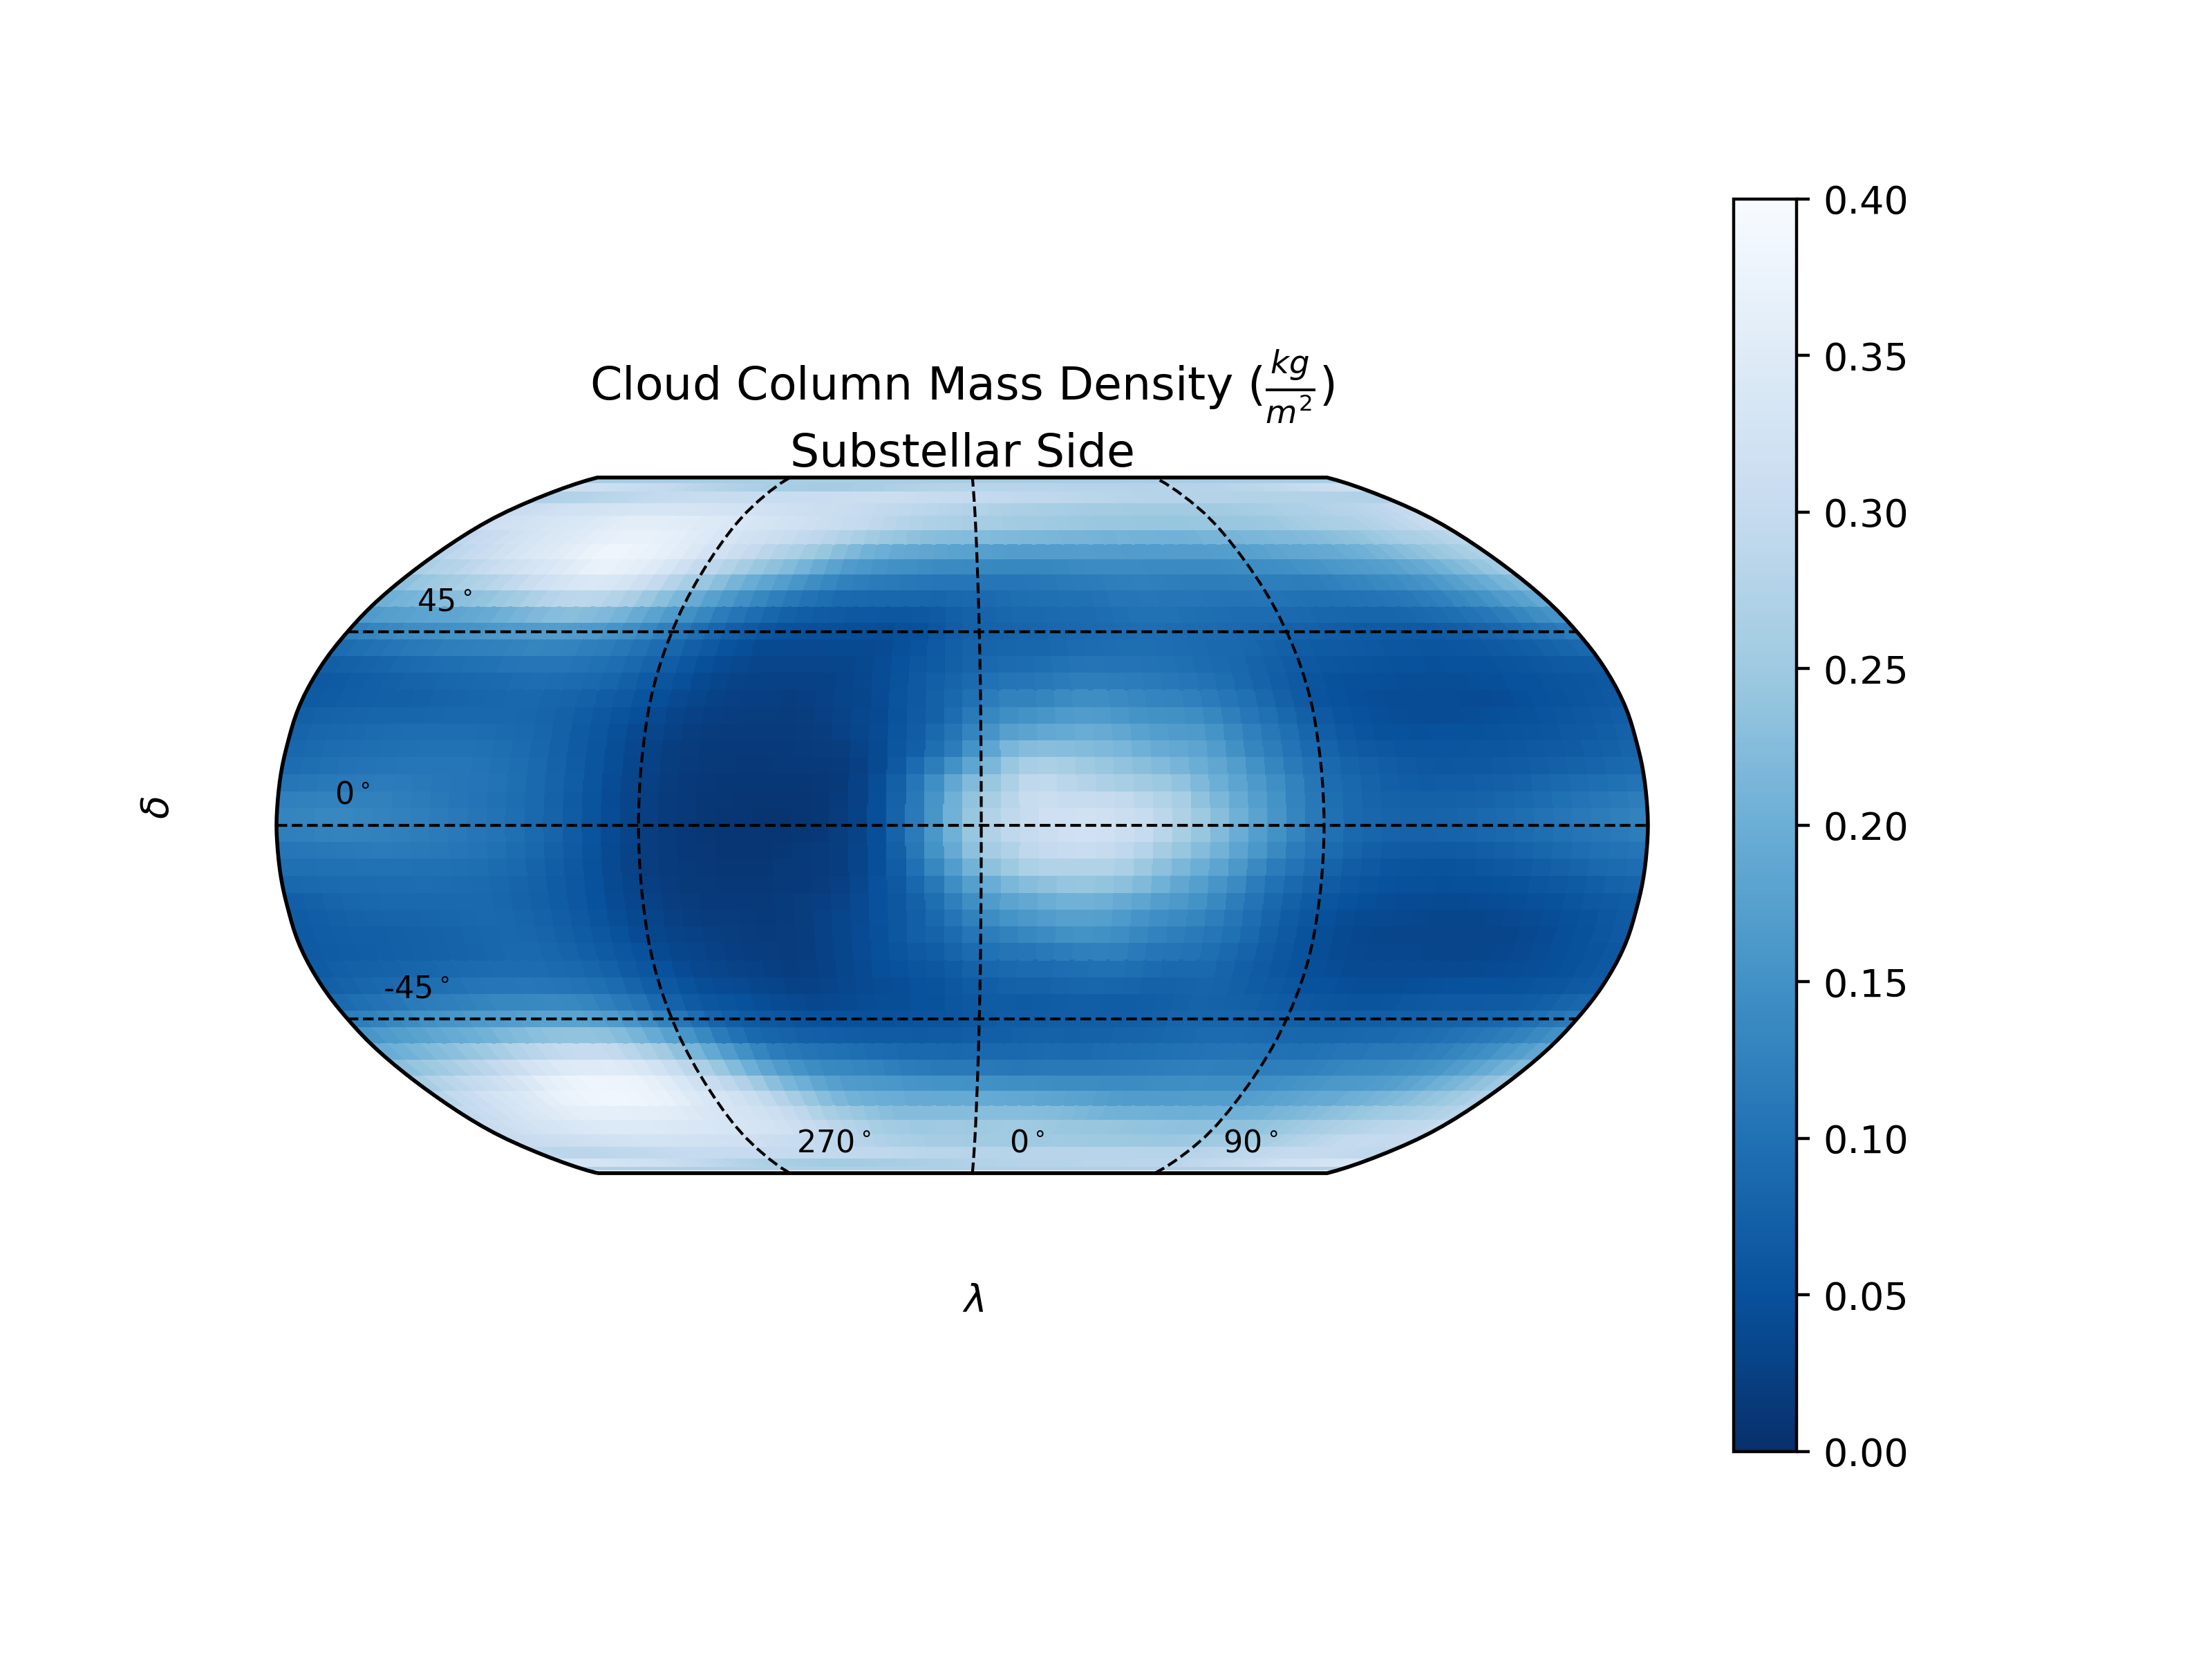
\includegraphics[width=0.8\textwidth]{models/cloud_map.png}
        \end{figure}
        \vspace{-2EM}
        \begin{figure}
        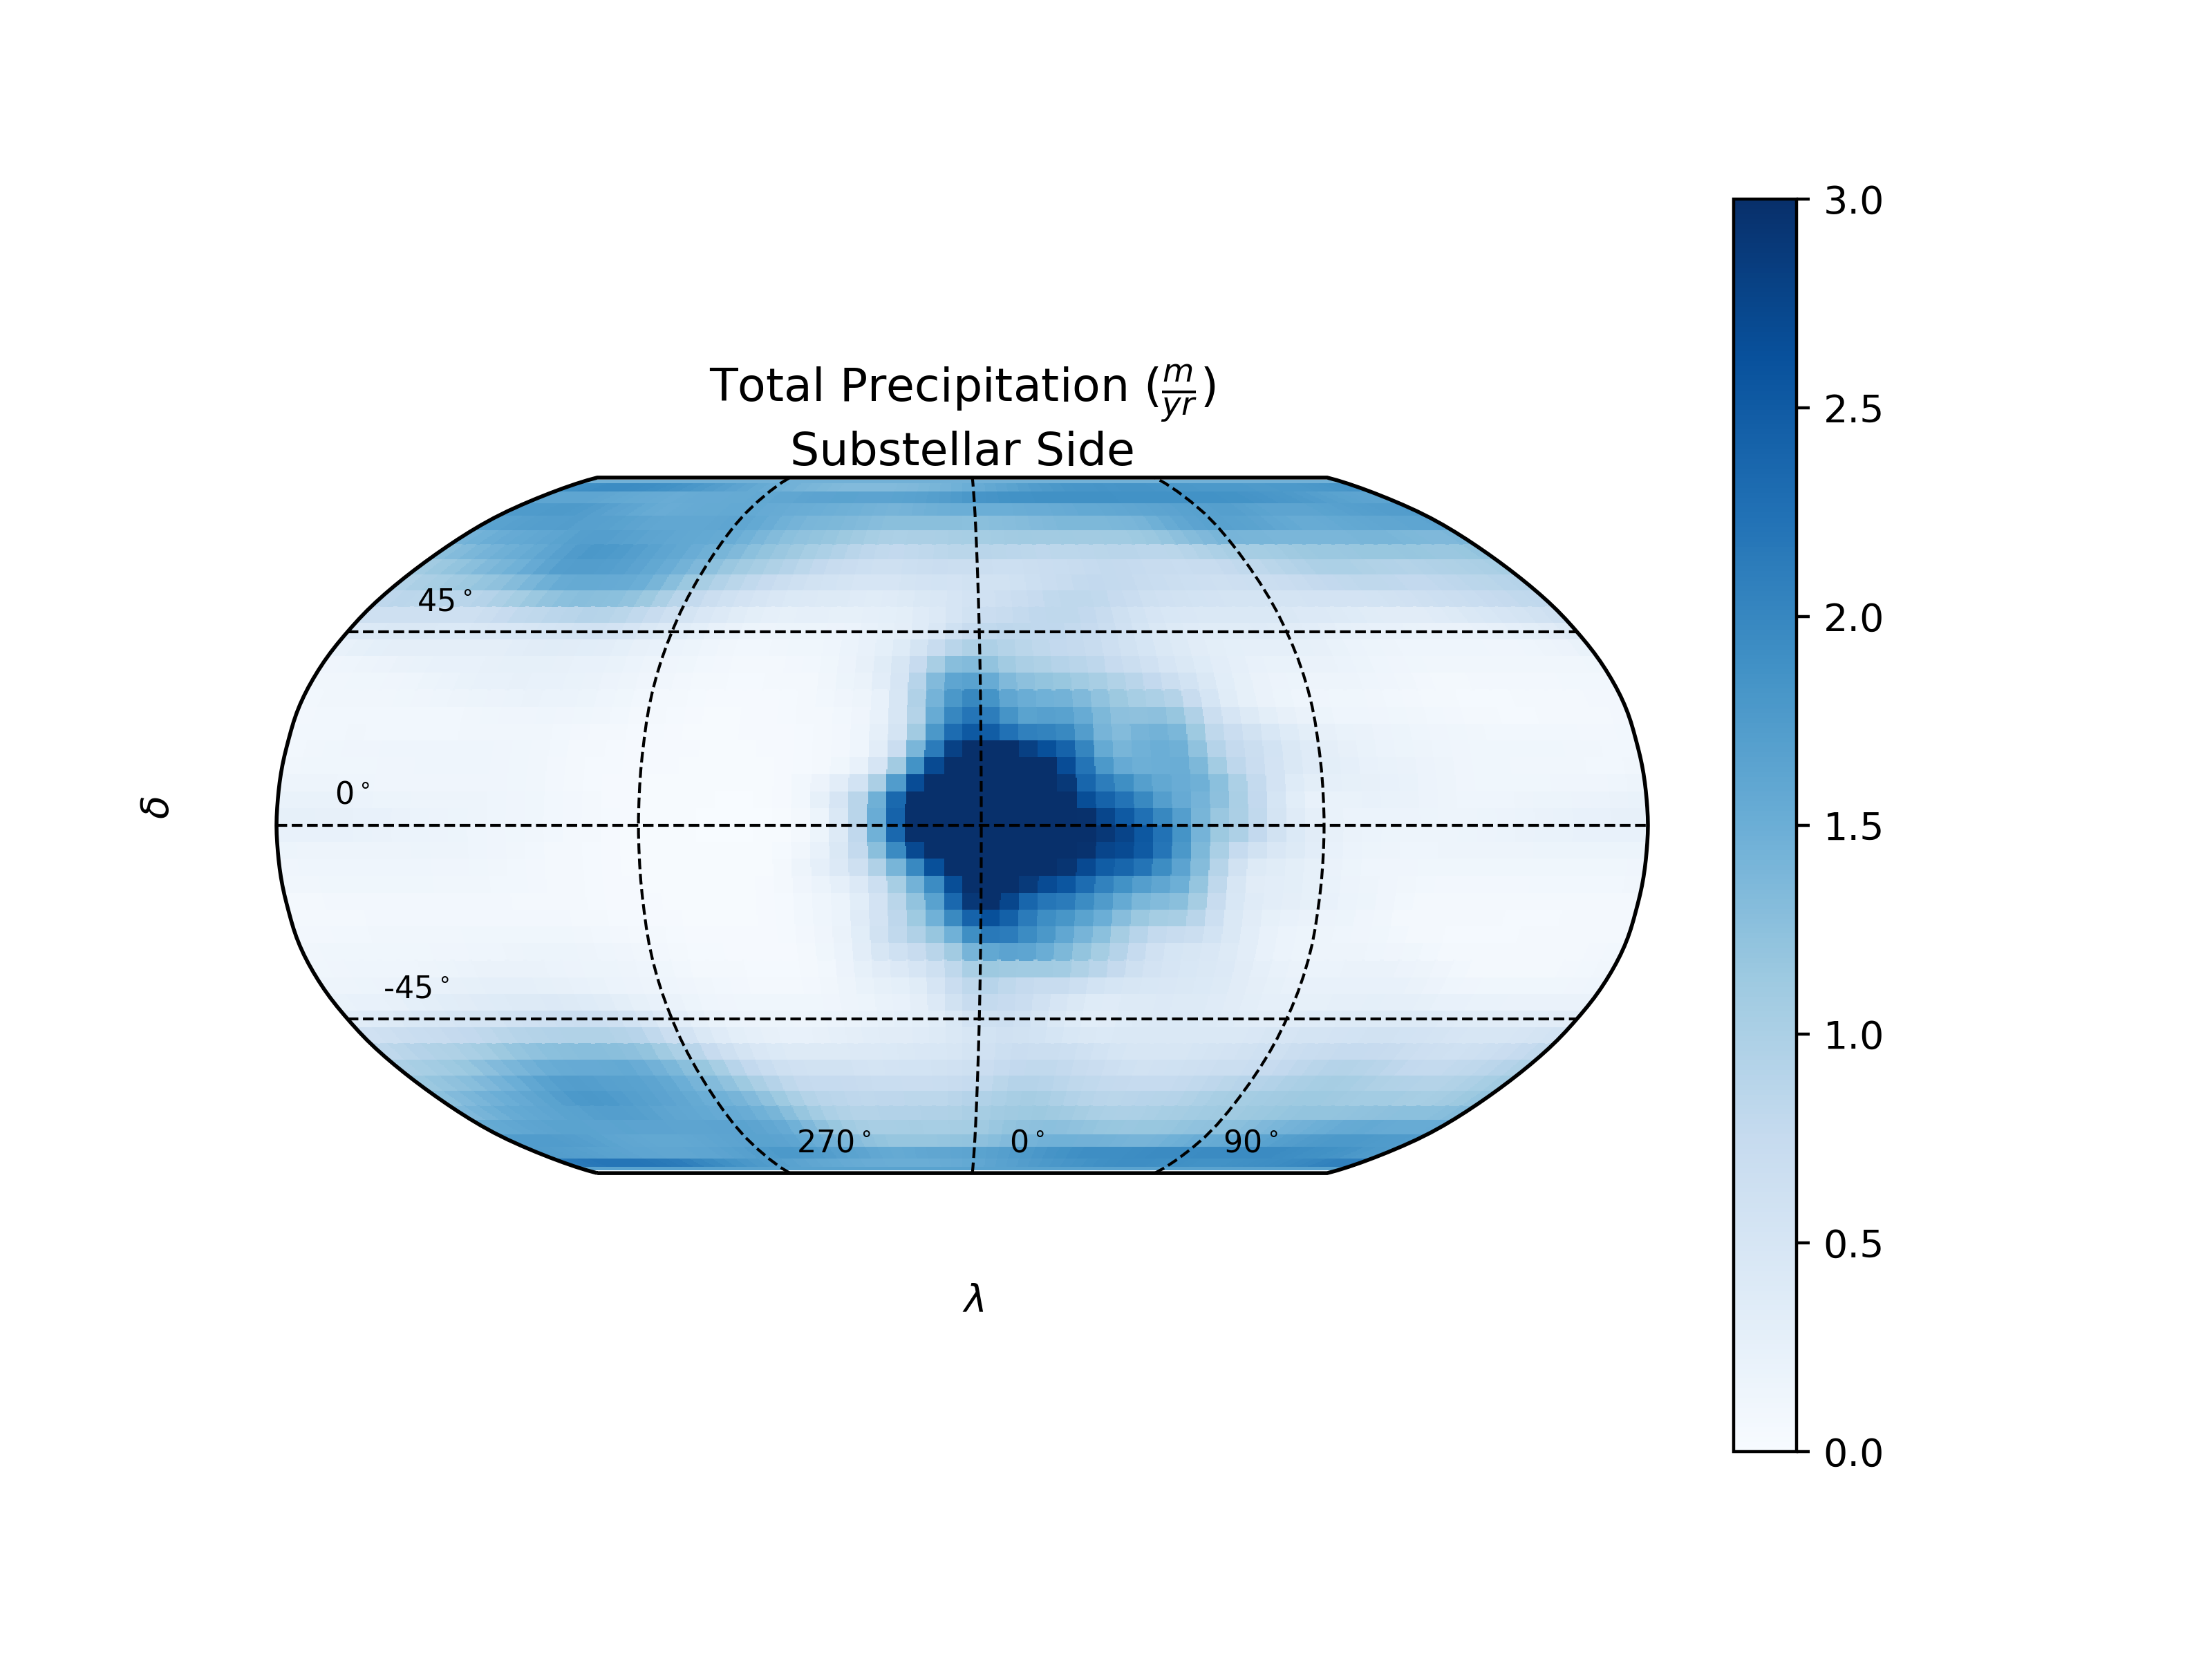
\includegraphics[width=0.8\textwidth]{models/precipitation_map.png}
        \end{figure}
    \column{0.5\textwidth}
        % \vpsace{-1EM}   
        {\tiny Slow rotator}
        \begin{figure}[topsep=0pt, partopsep=0pt]
        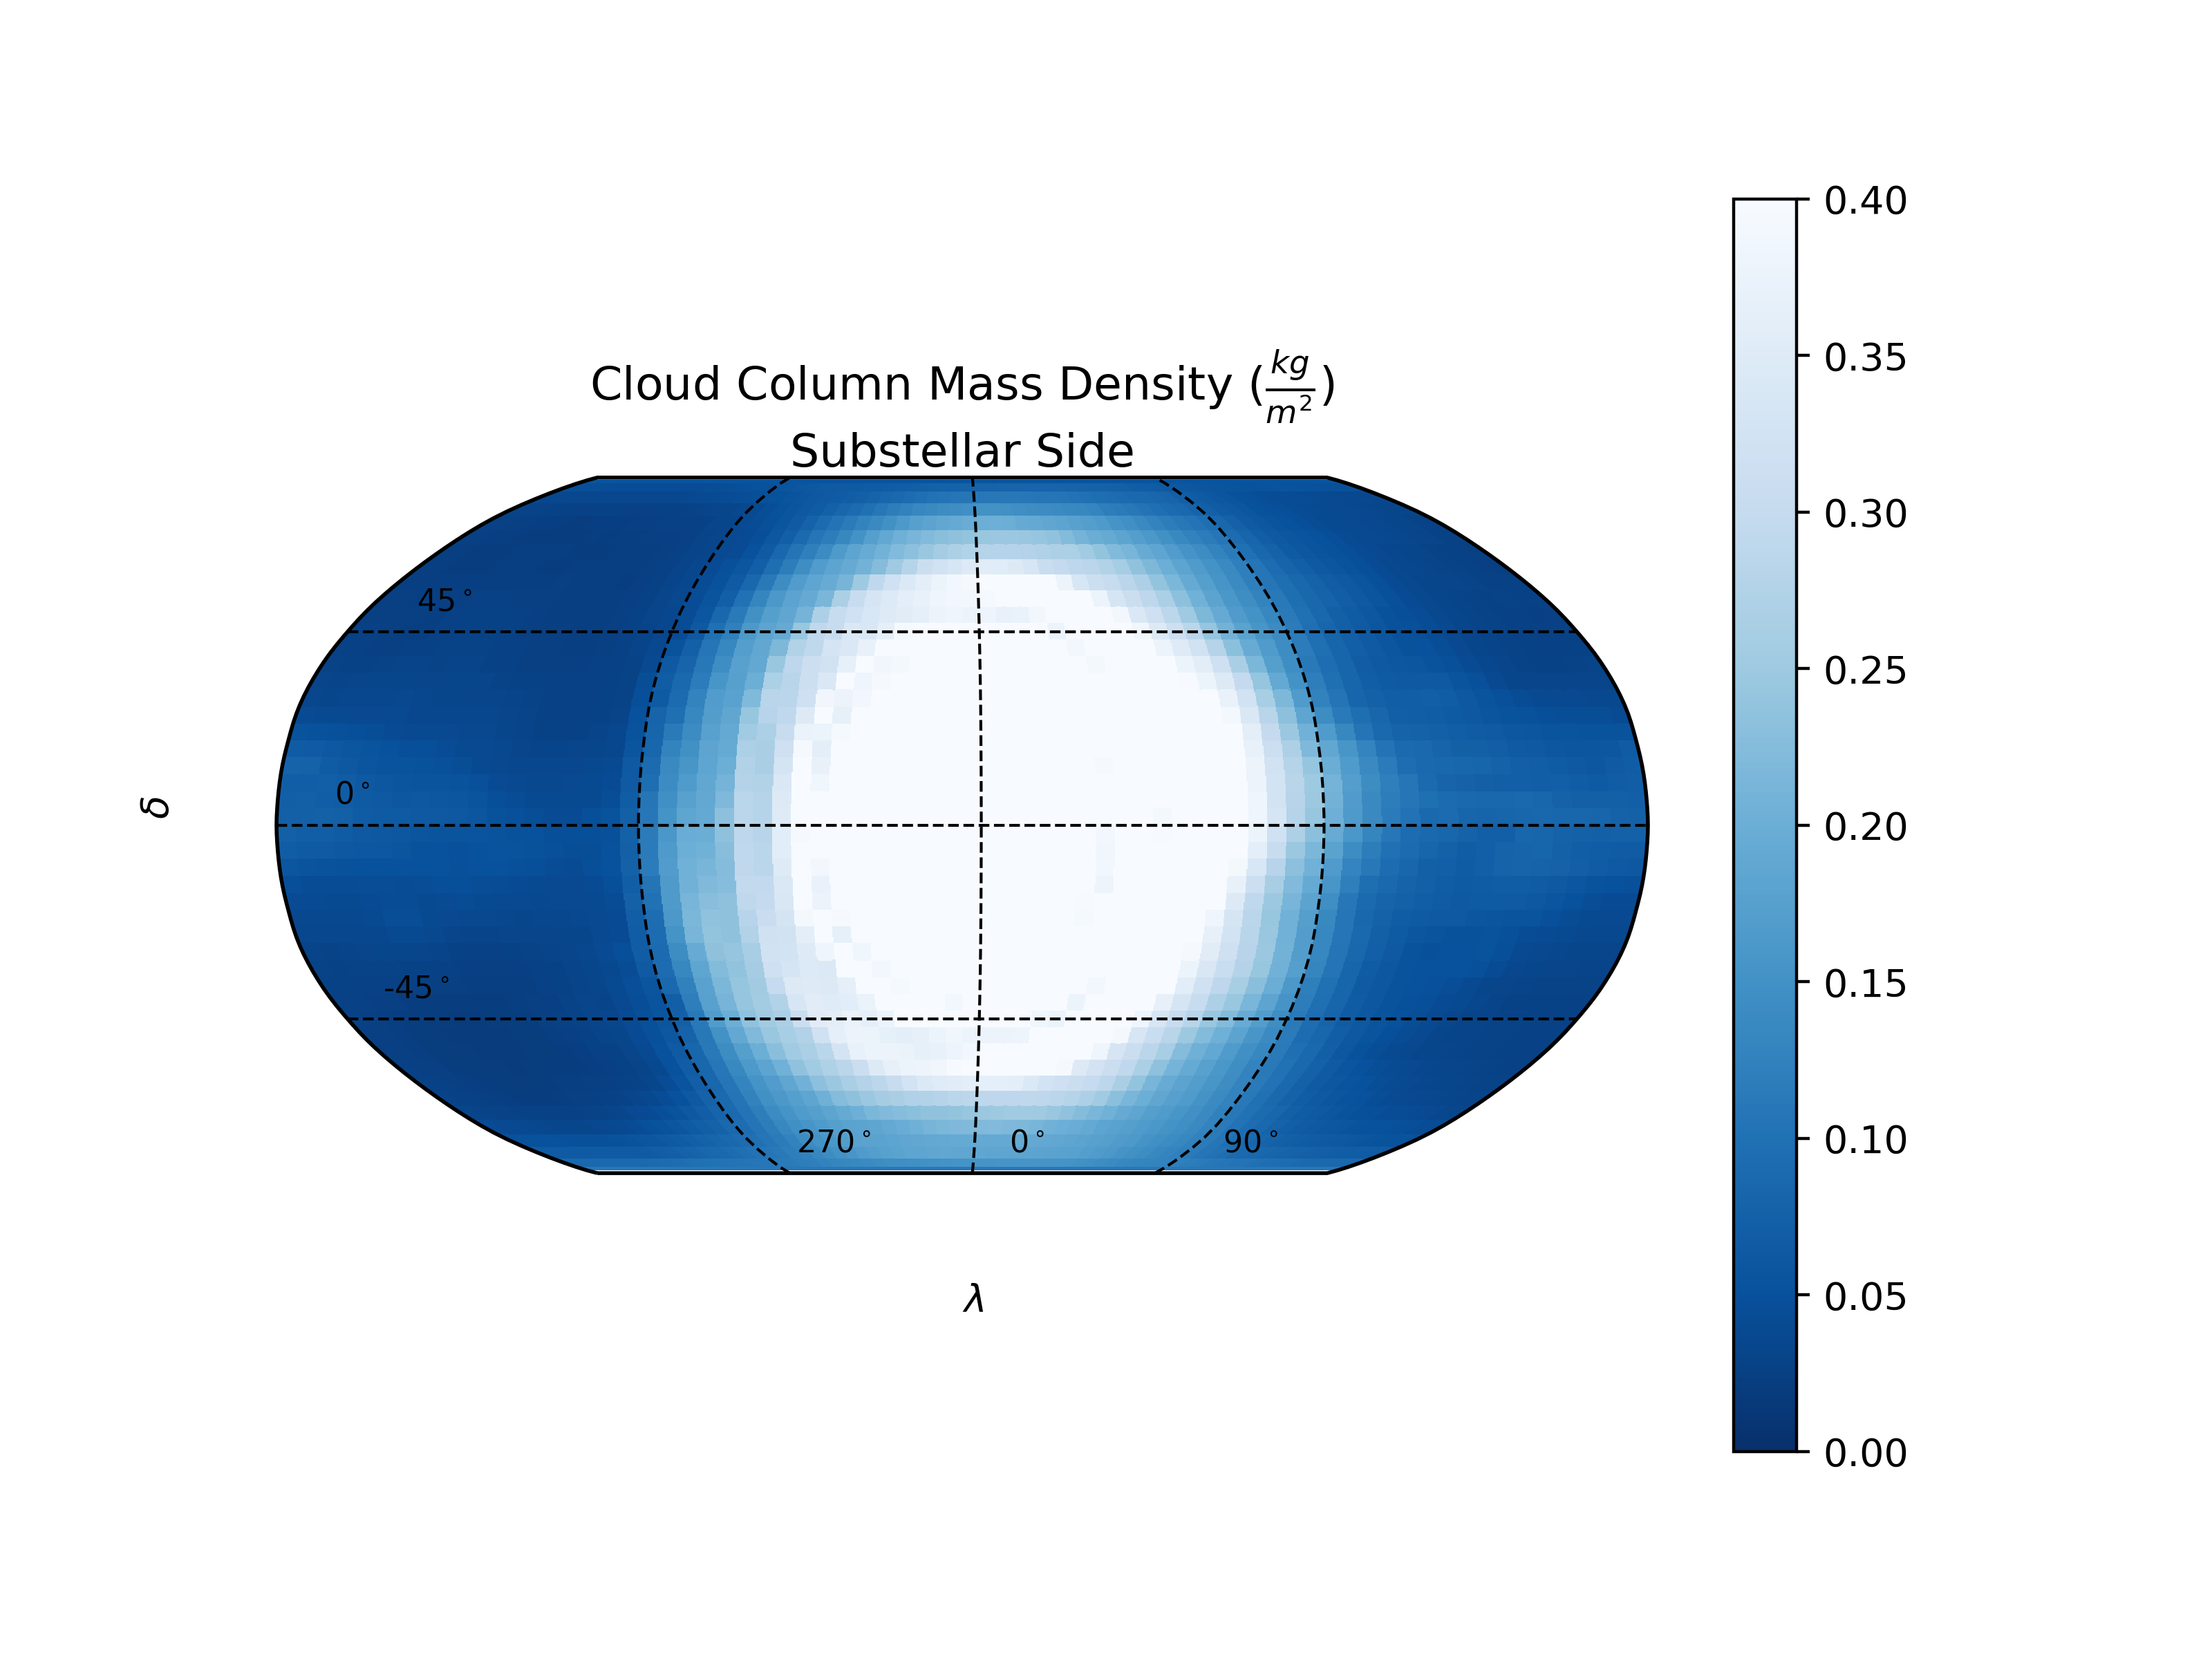
\includegraphics[width=0.8\textwidth]{models/slow_rotator_cloud_map.png}
        \end{figure}
        \vspace{-2EM}
        {\tiny 1bar\chem{N_2} 1bar\chem{CO_2}}
        \begin{figure}
        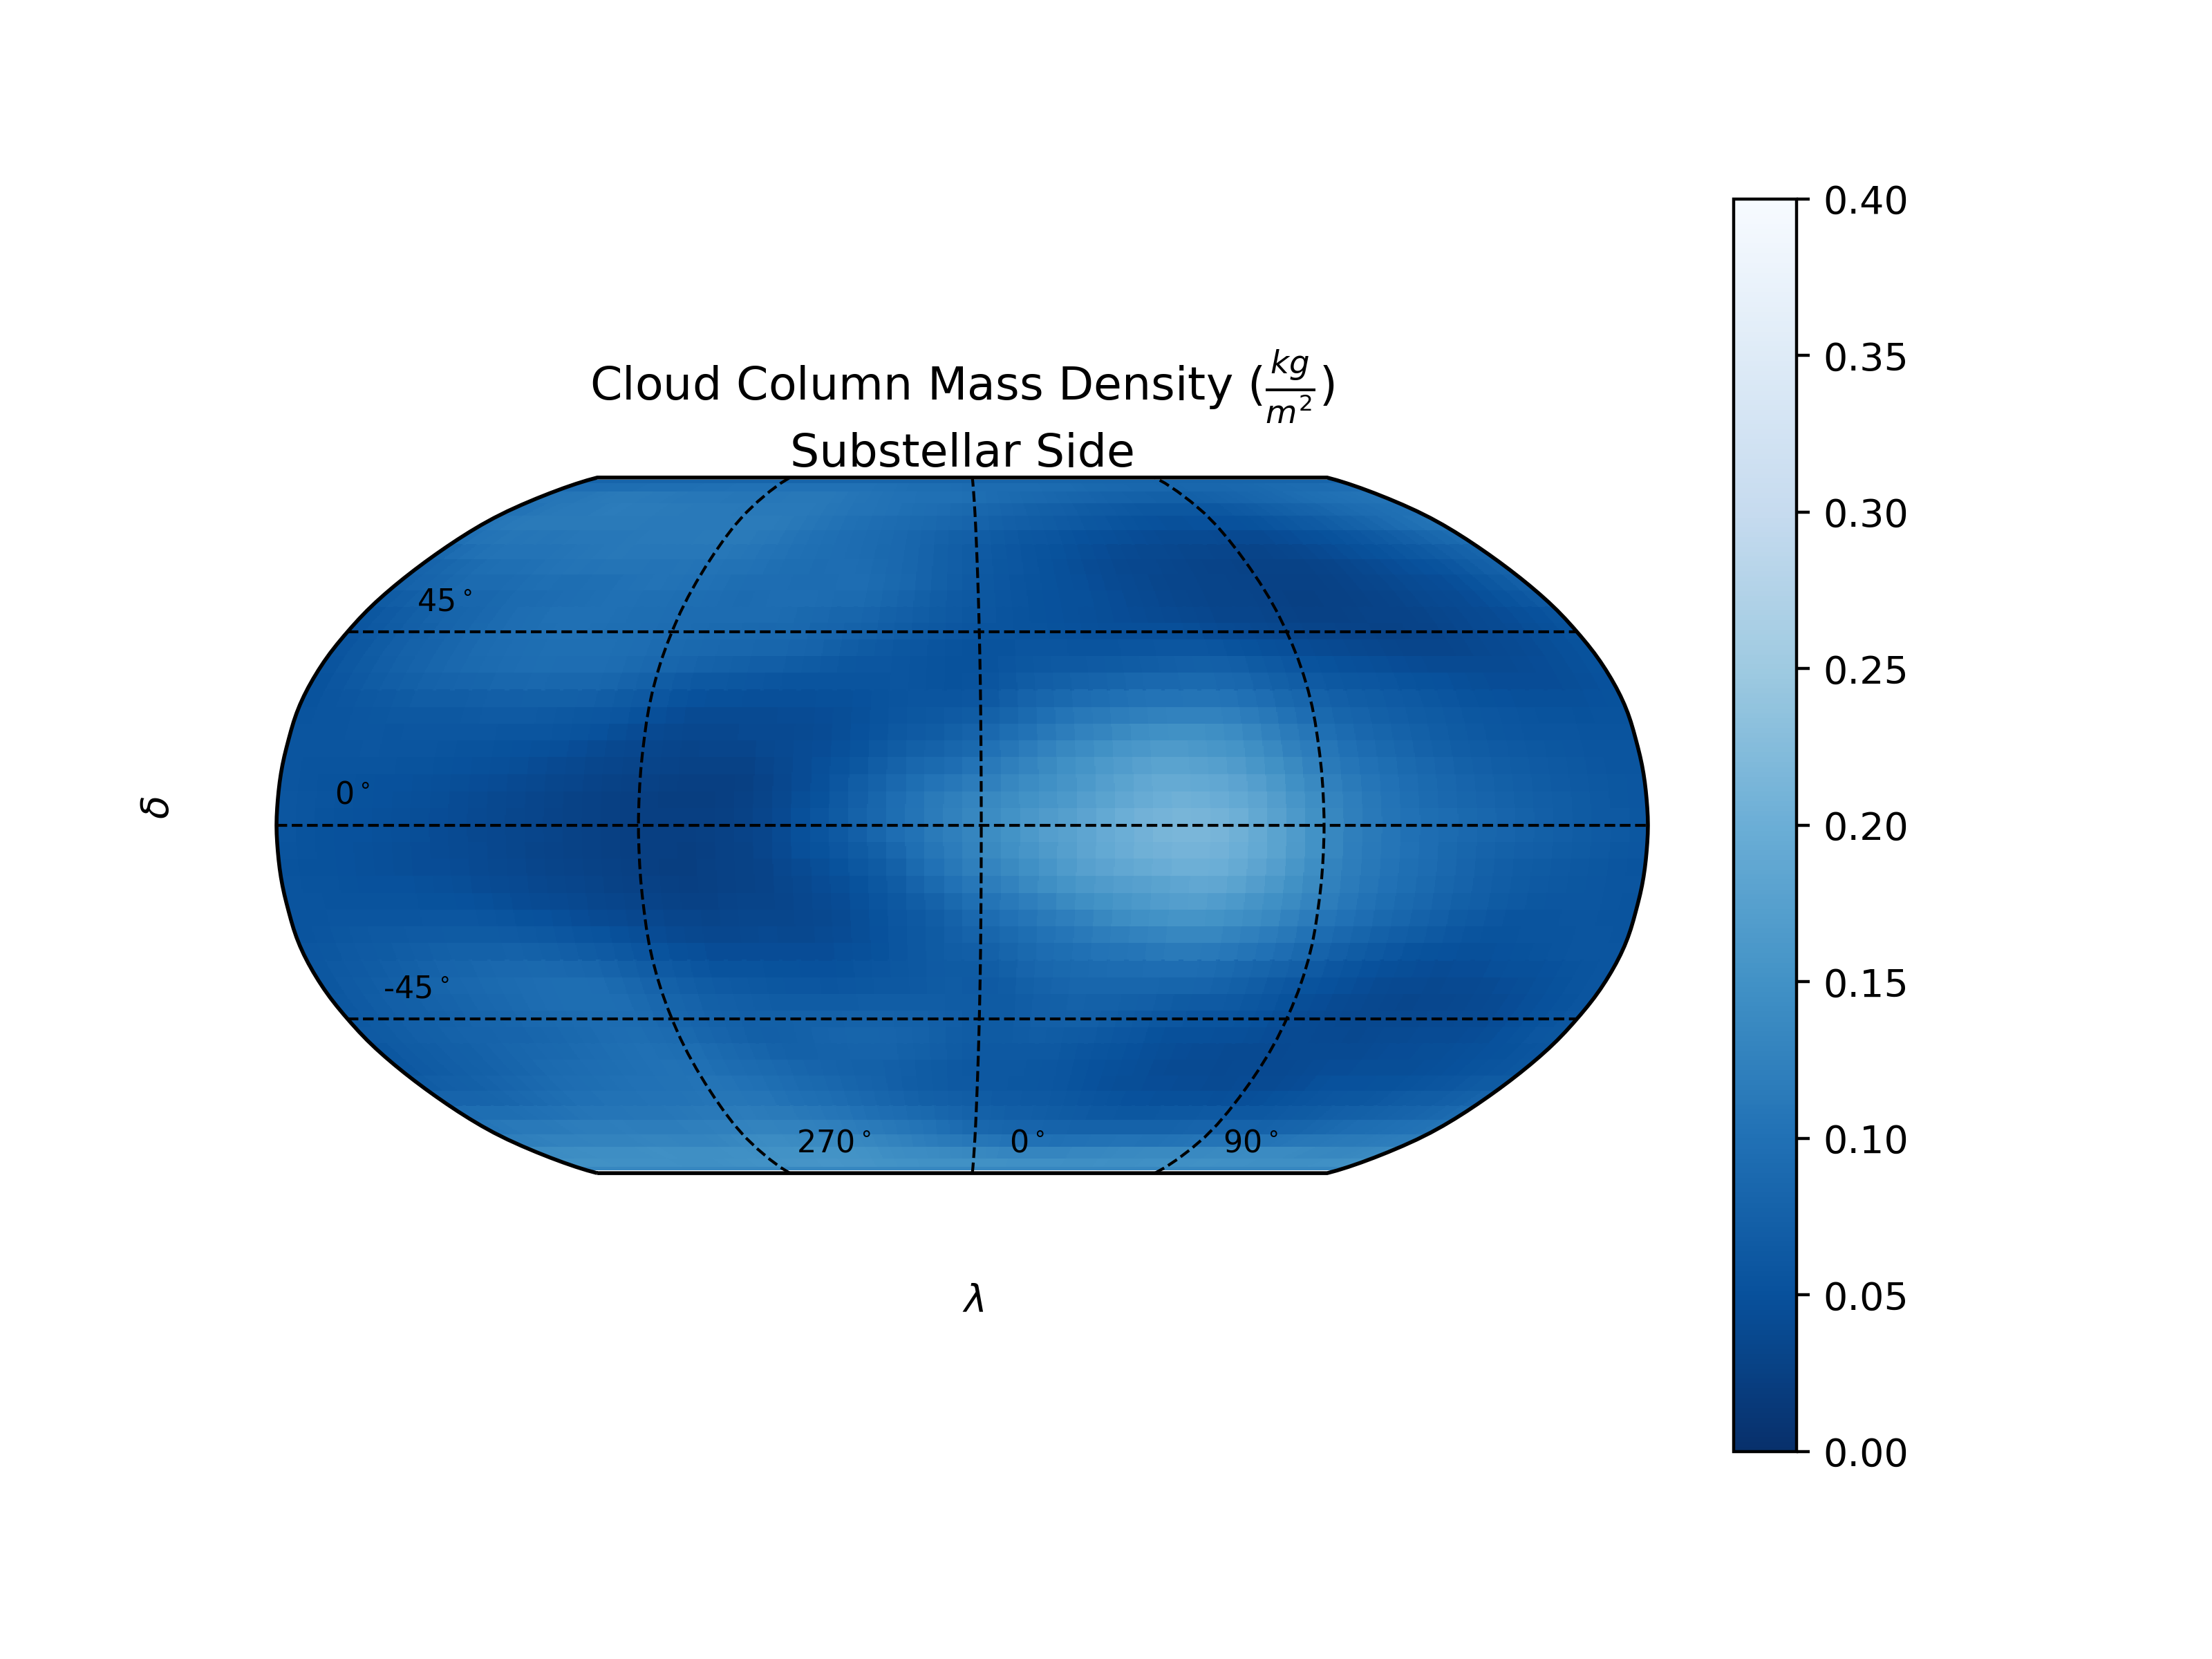
\includegraphics[width=0.8\textwidth]{models/hot_cloud_map.png}
        \end{figure}
        % \vpspace{-2.5EM}
    \end{columns}
\end{frame}

\section{Methods}
\subsection{Adding layers}

\begin{frame}
    \frametitle{TRAPPIST-1 e climate models are too short for radiative transfer models}
    \begin{columns}
    \column{0.3\textwidth}
        {\small 1bar \chem{N_2}
        
        0.4bar \chem{CO_2}
        
        Model top: 1mb

        Added top: $10^{-3}$mb}
    \column{0.7\textwidth}
        \begin{figure}
            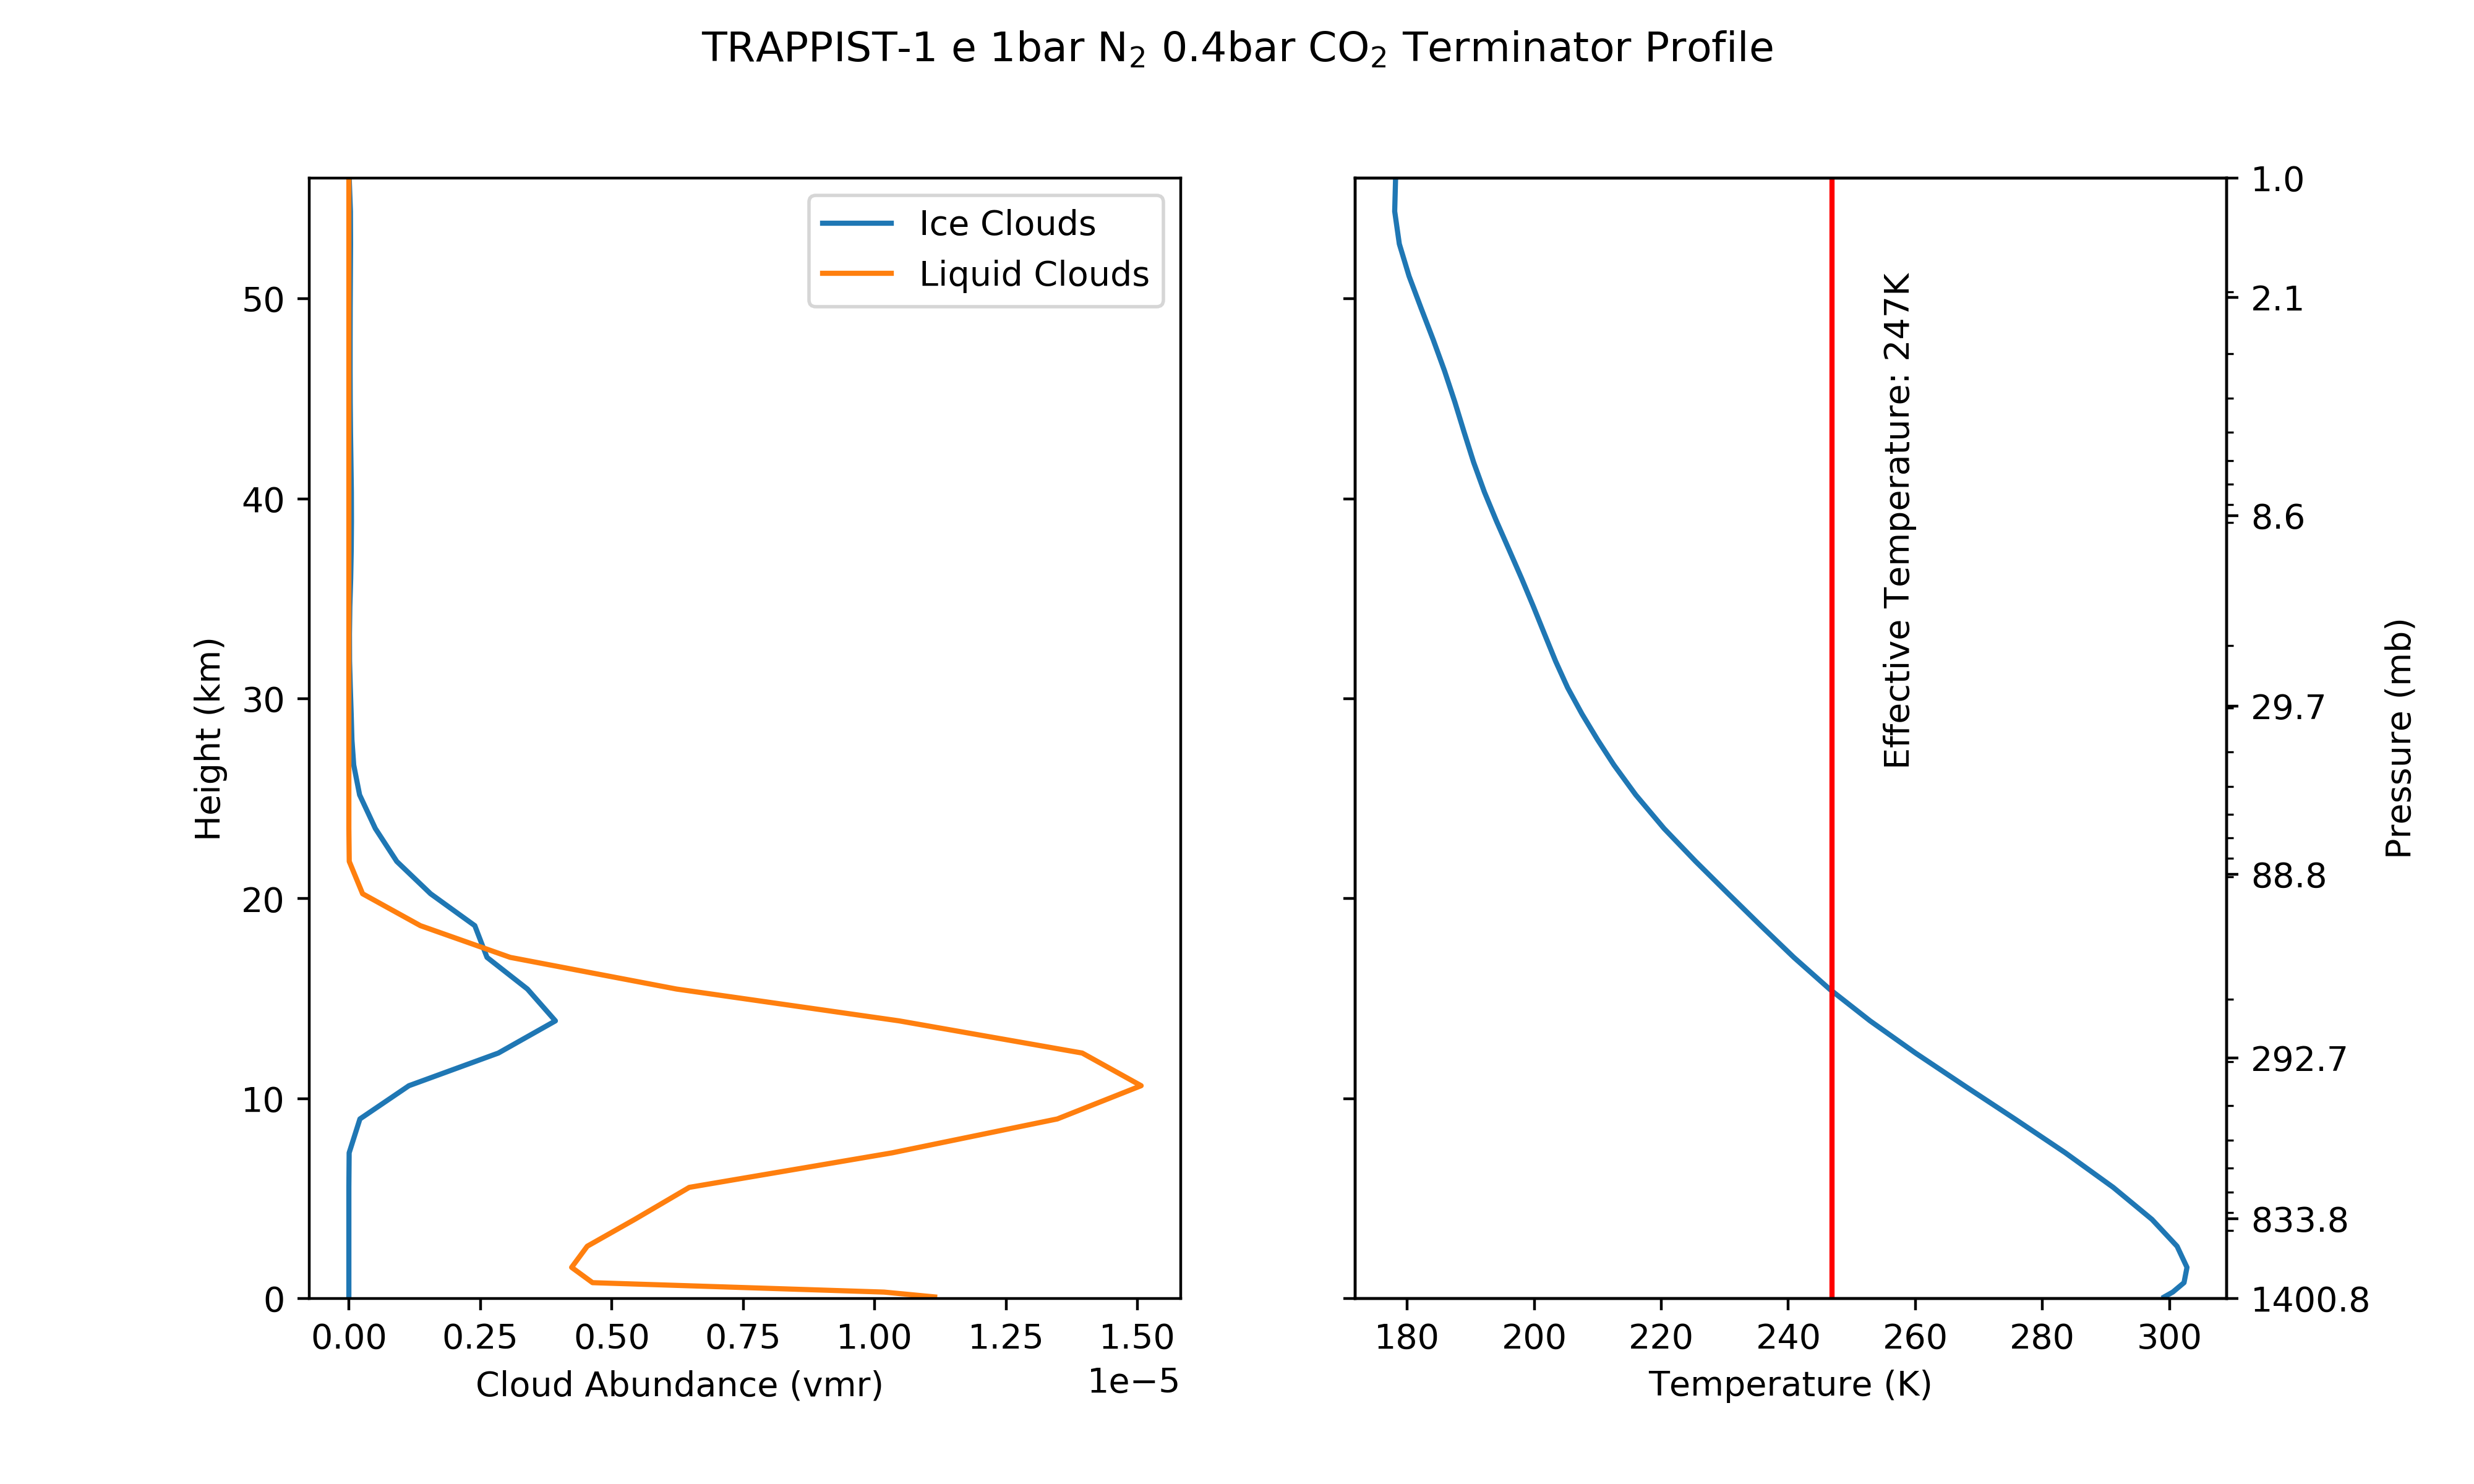
\includegraphics[width=\textwidth]{models/atmosphere_profile.png}
        \end{figure}
    \end{columns}
\end{frame}

\begin{frame}
    \frametitle{TRAPPIST-1 e climate models are too short for radiative transfer models}
    \begin{columns}
    \column{0.3\textwidth}
        {\small 1bar \chem{N_2}
        
        0.4bar \chem{CO_2}
        
        Model top: 1mb

        Added top: $10^{-3}$mb}
    \column{0.7\textwidth}
        \begin{figure}
            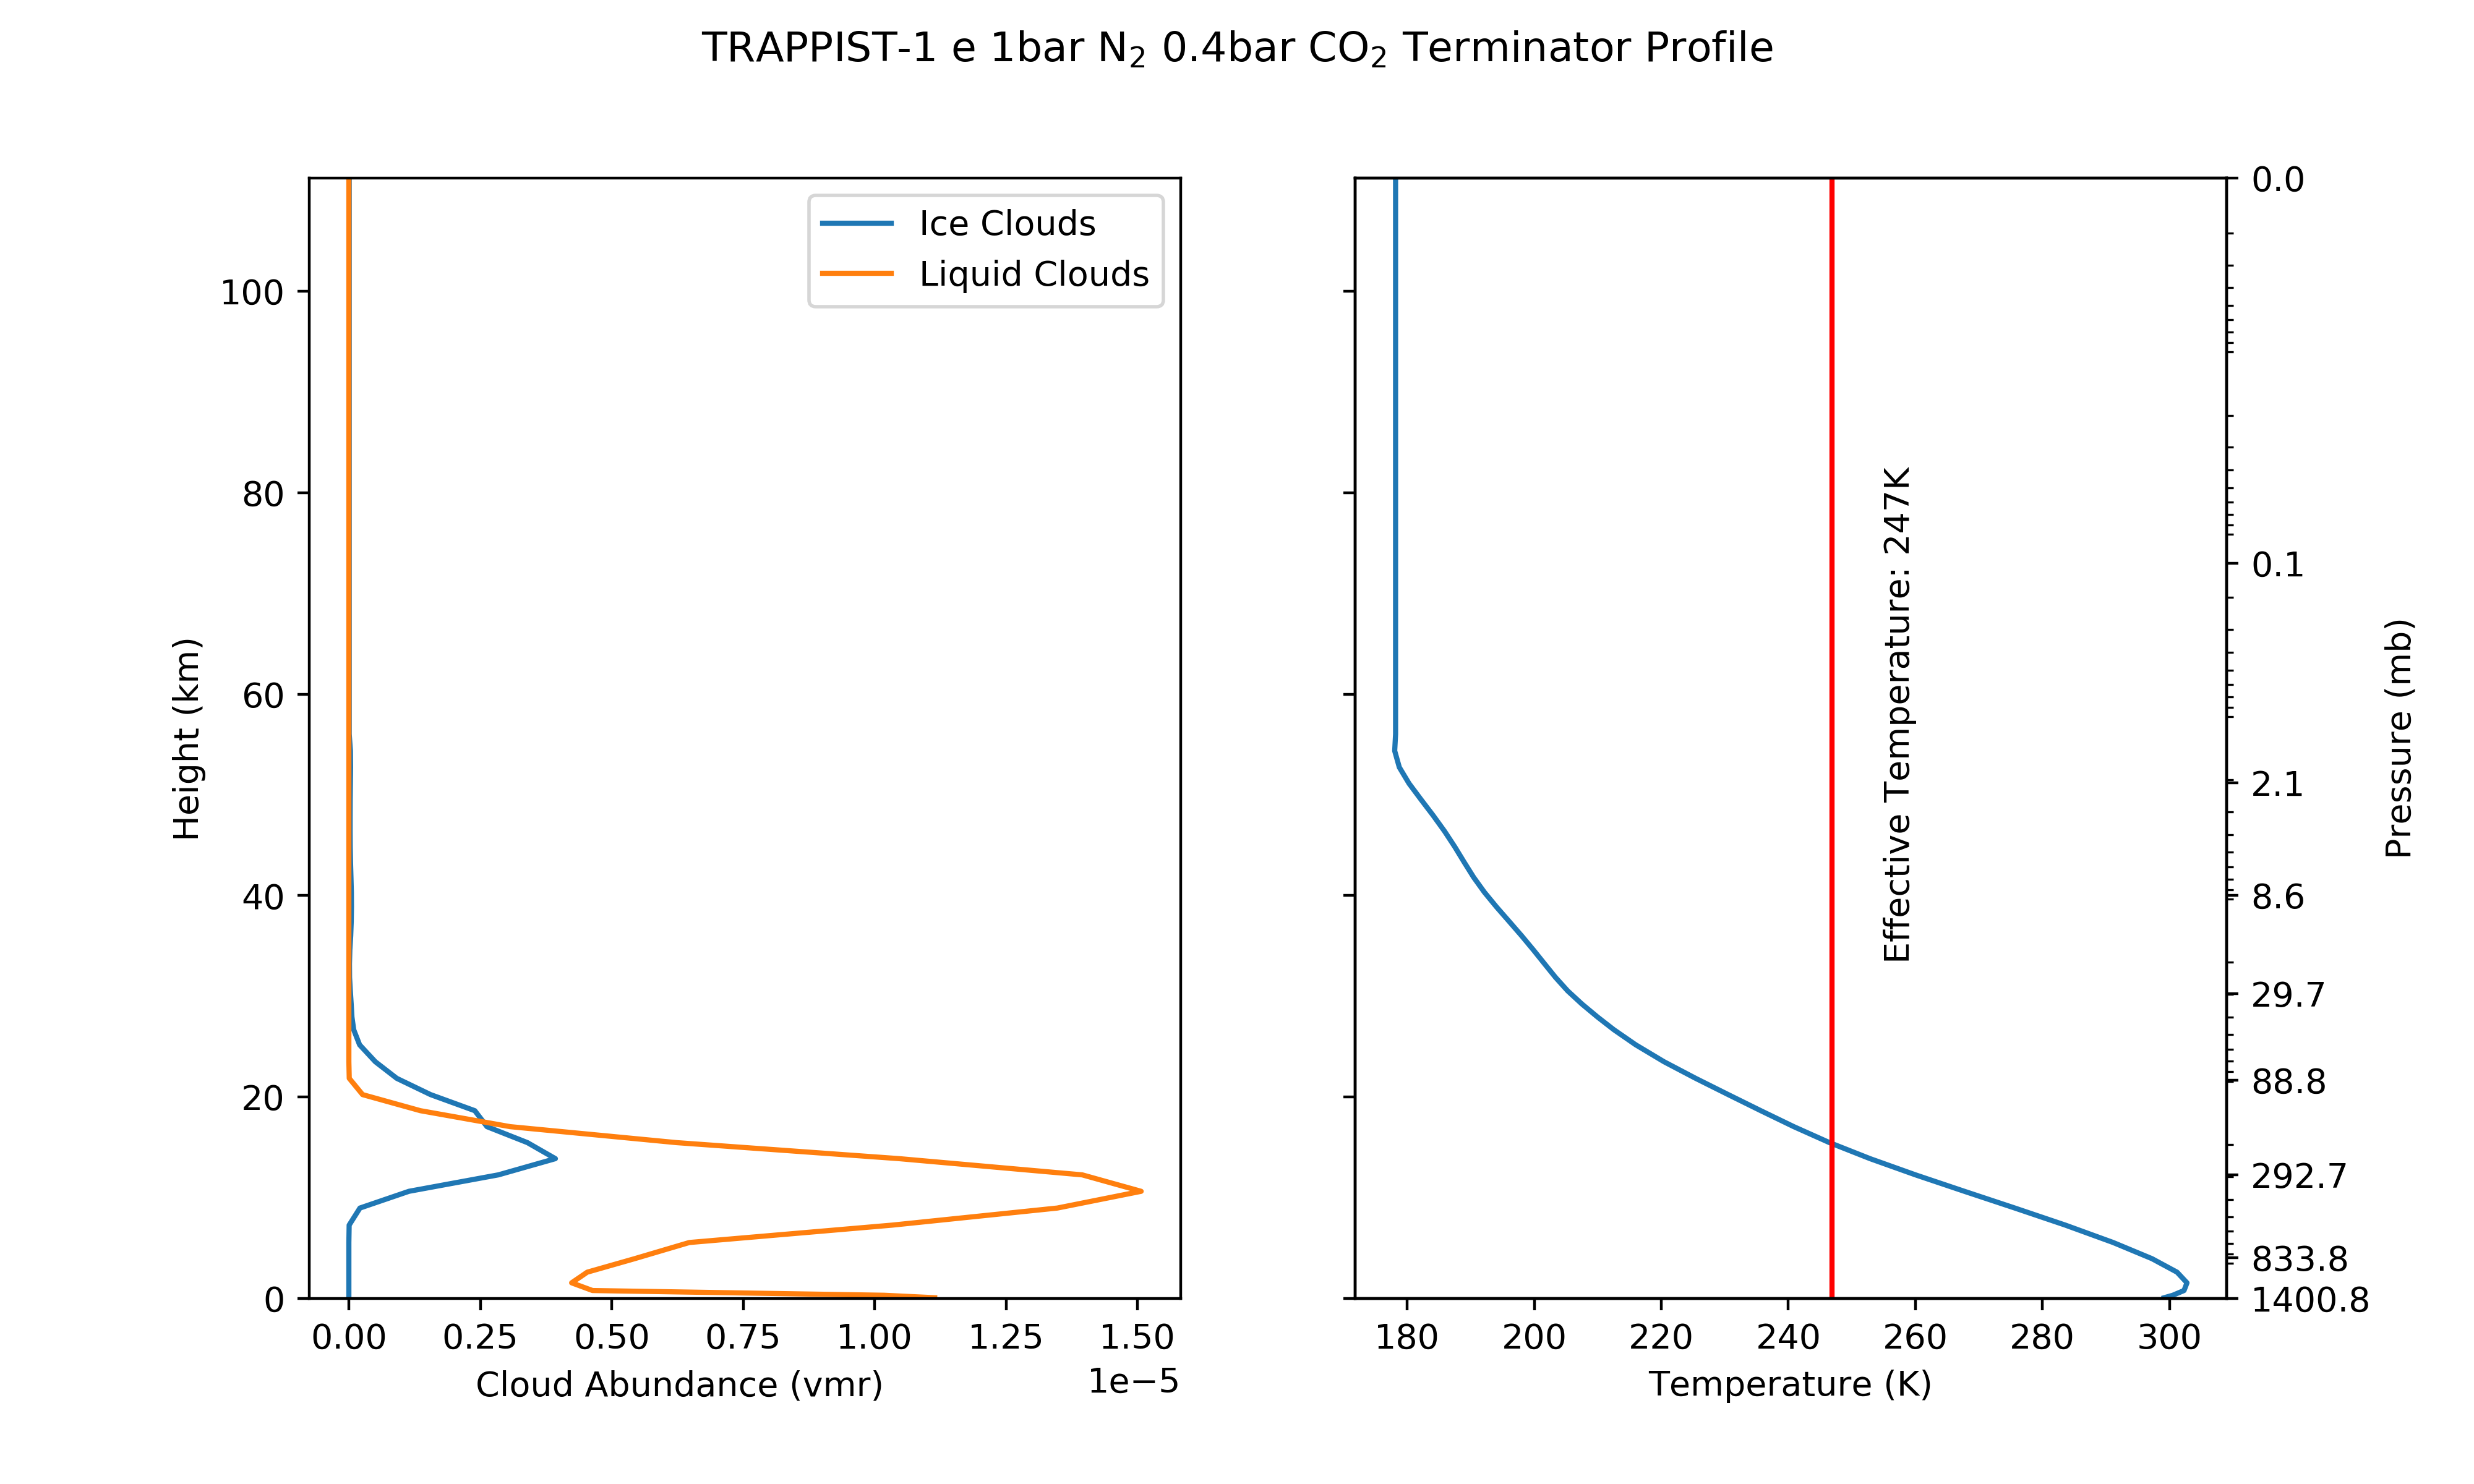
\includegraphics[width=\textwidth]{models/atmosphere_profile_tall.png}
        \end{figure}
    \end{columns}
\end{frame}

\subsection{Area weighted averaging}
\begin{frame}
    \frametitle{3D models must be reduced 1D profiles using a weighting scheme}
    For non-transits:
    \begin{figure}
        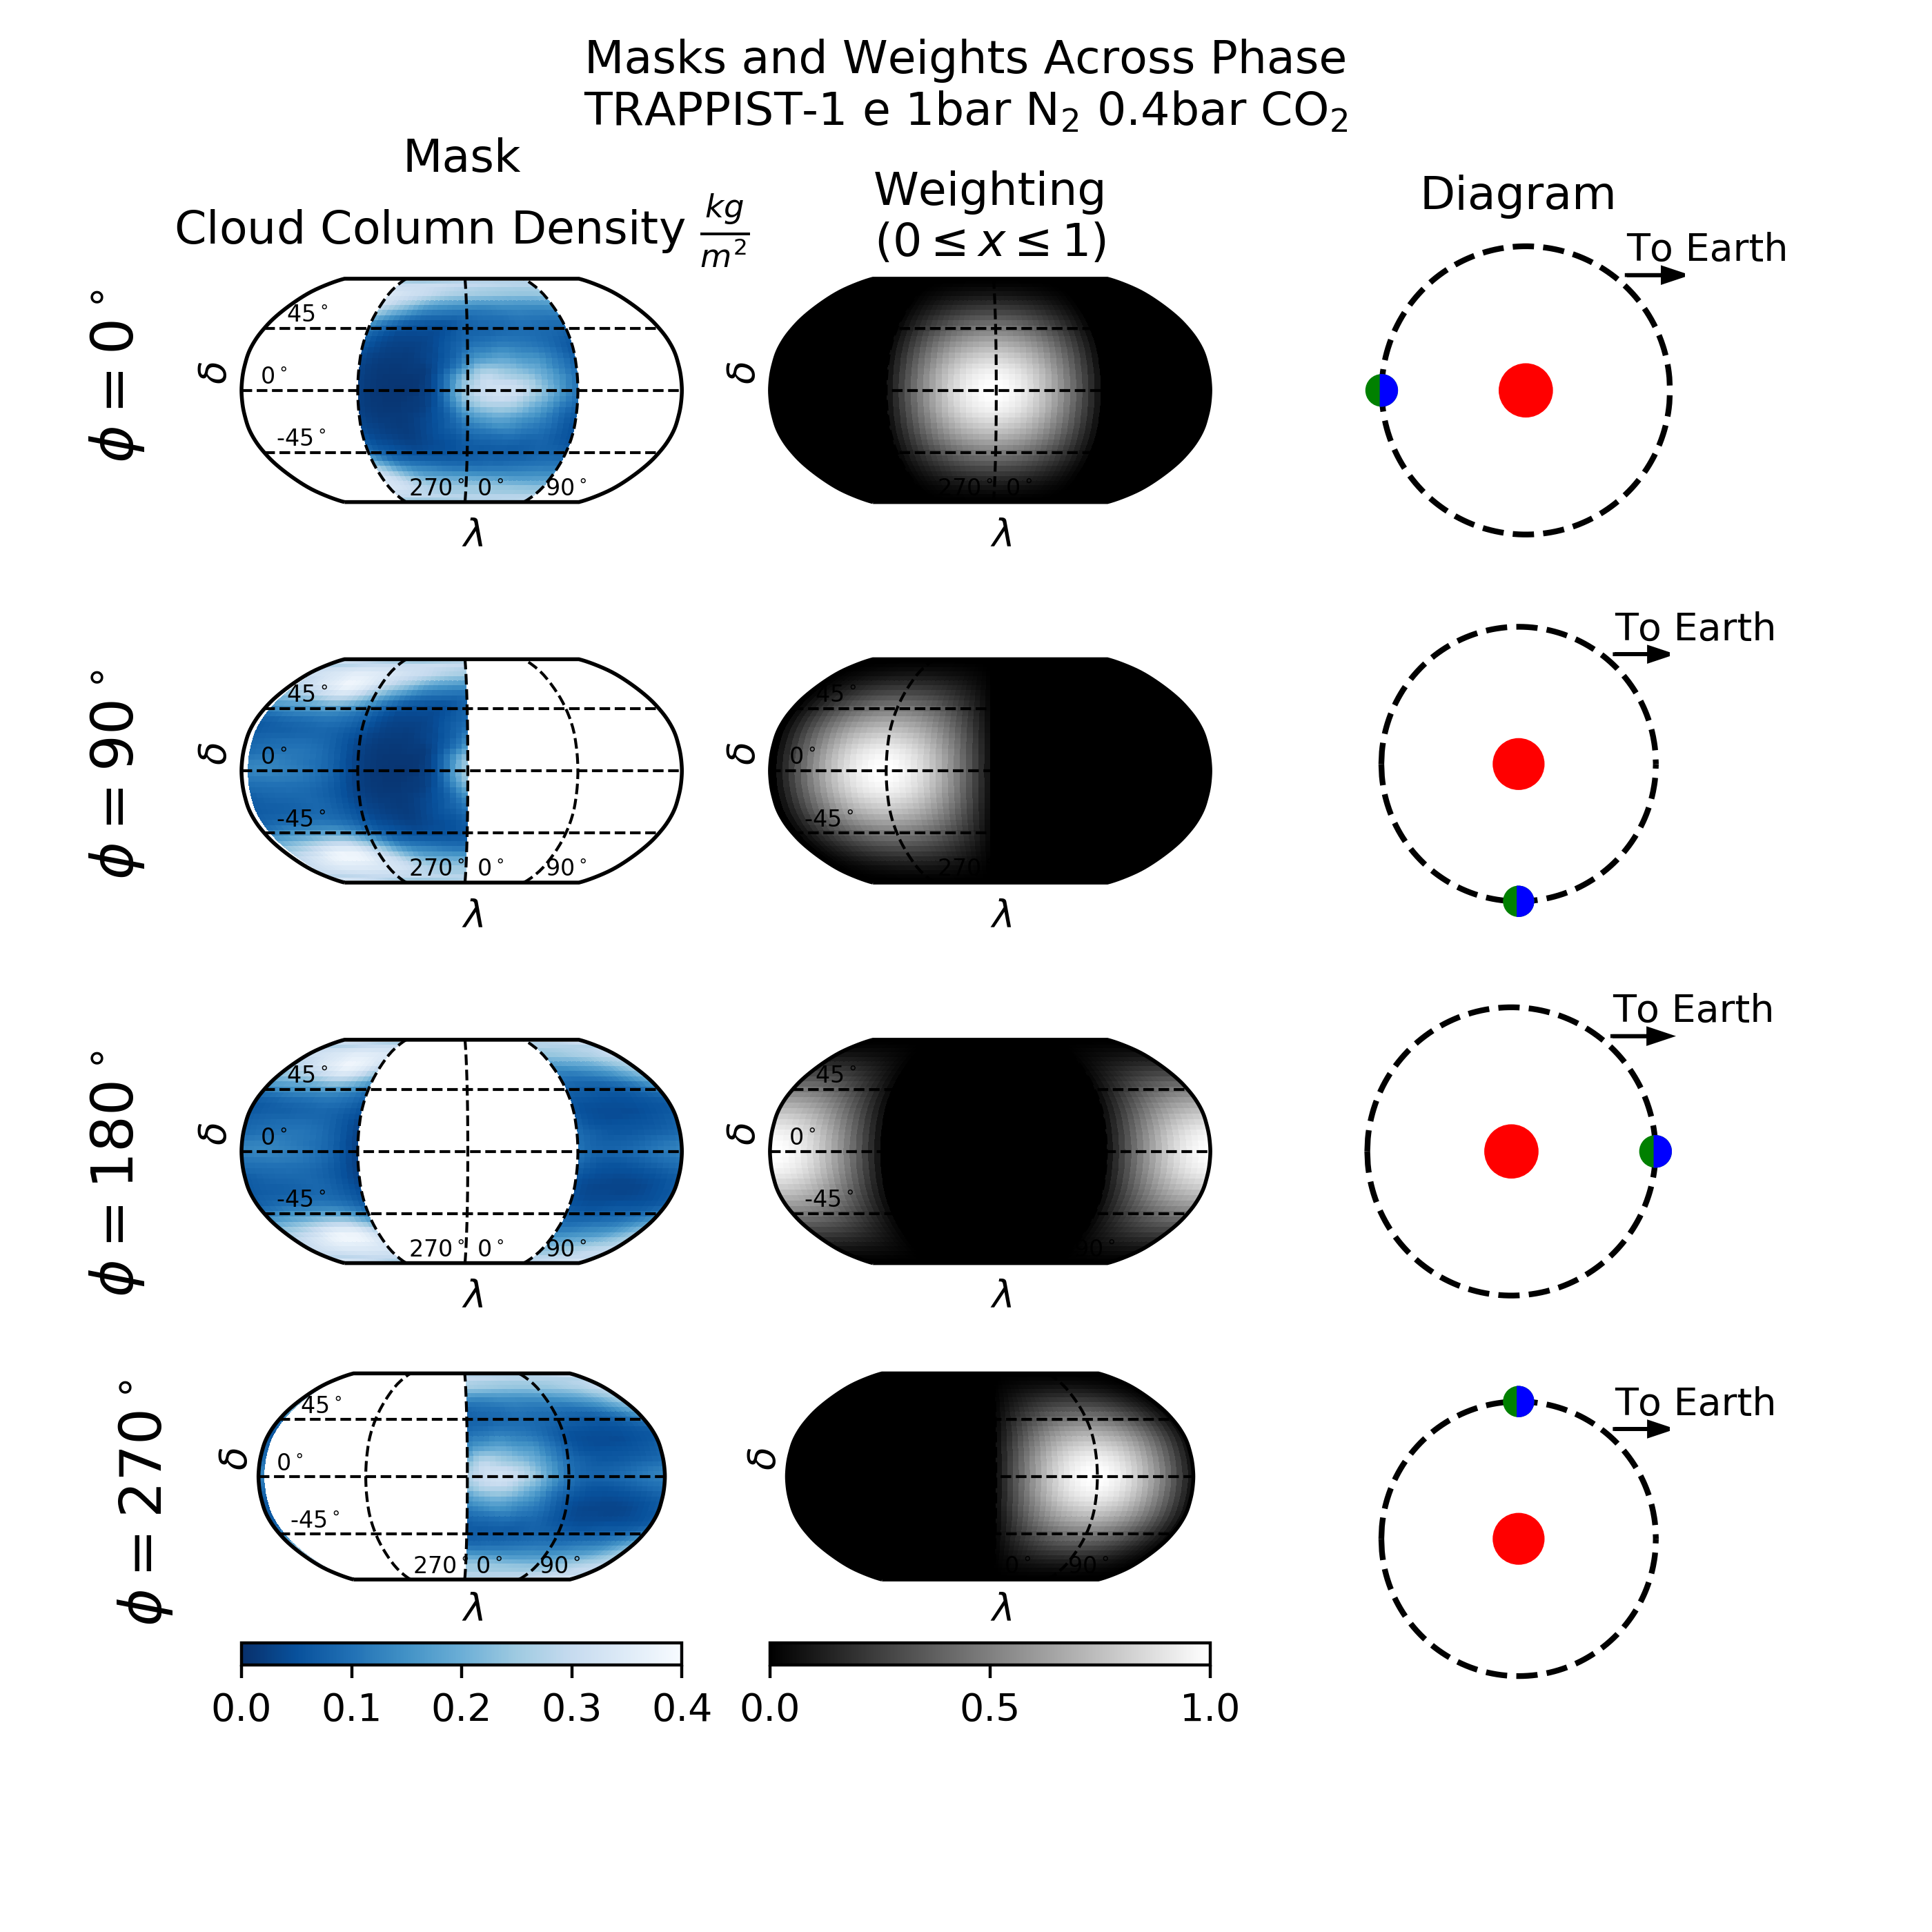
\includegraphics[height=0.8\textheight]{methods/phases_weights.png}
    \end{figure}
\end{frame}

\begin{frame}
    \frametitle{3D models must be reduced 1D profiles using a weighting scheme}
    For transits:
    \begin{figure}
        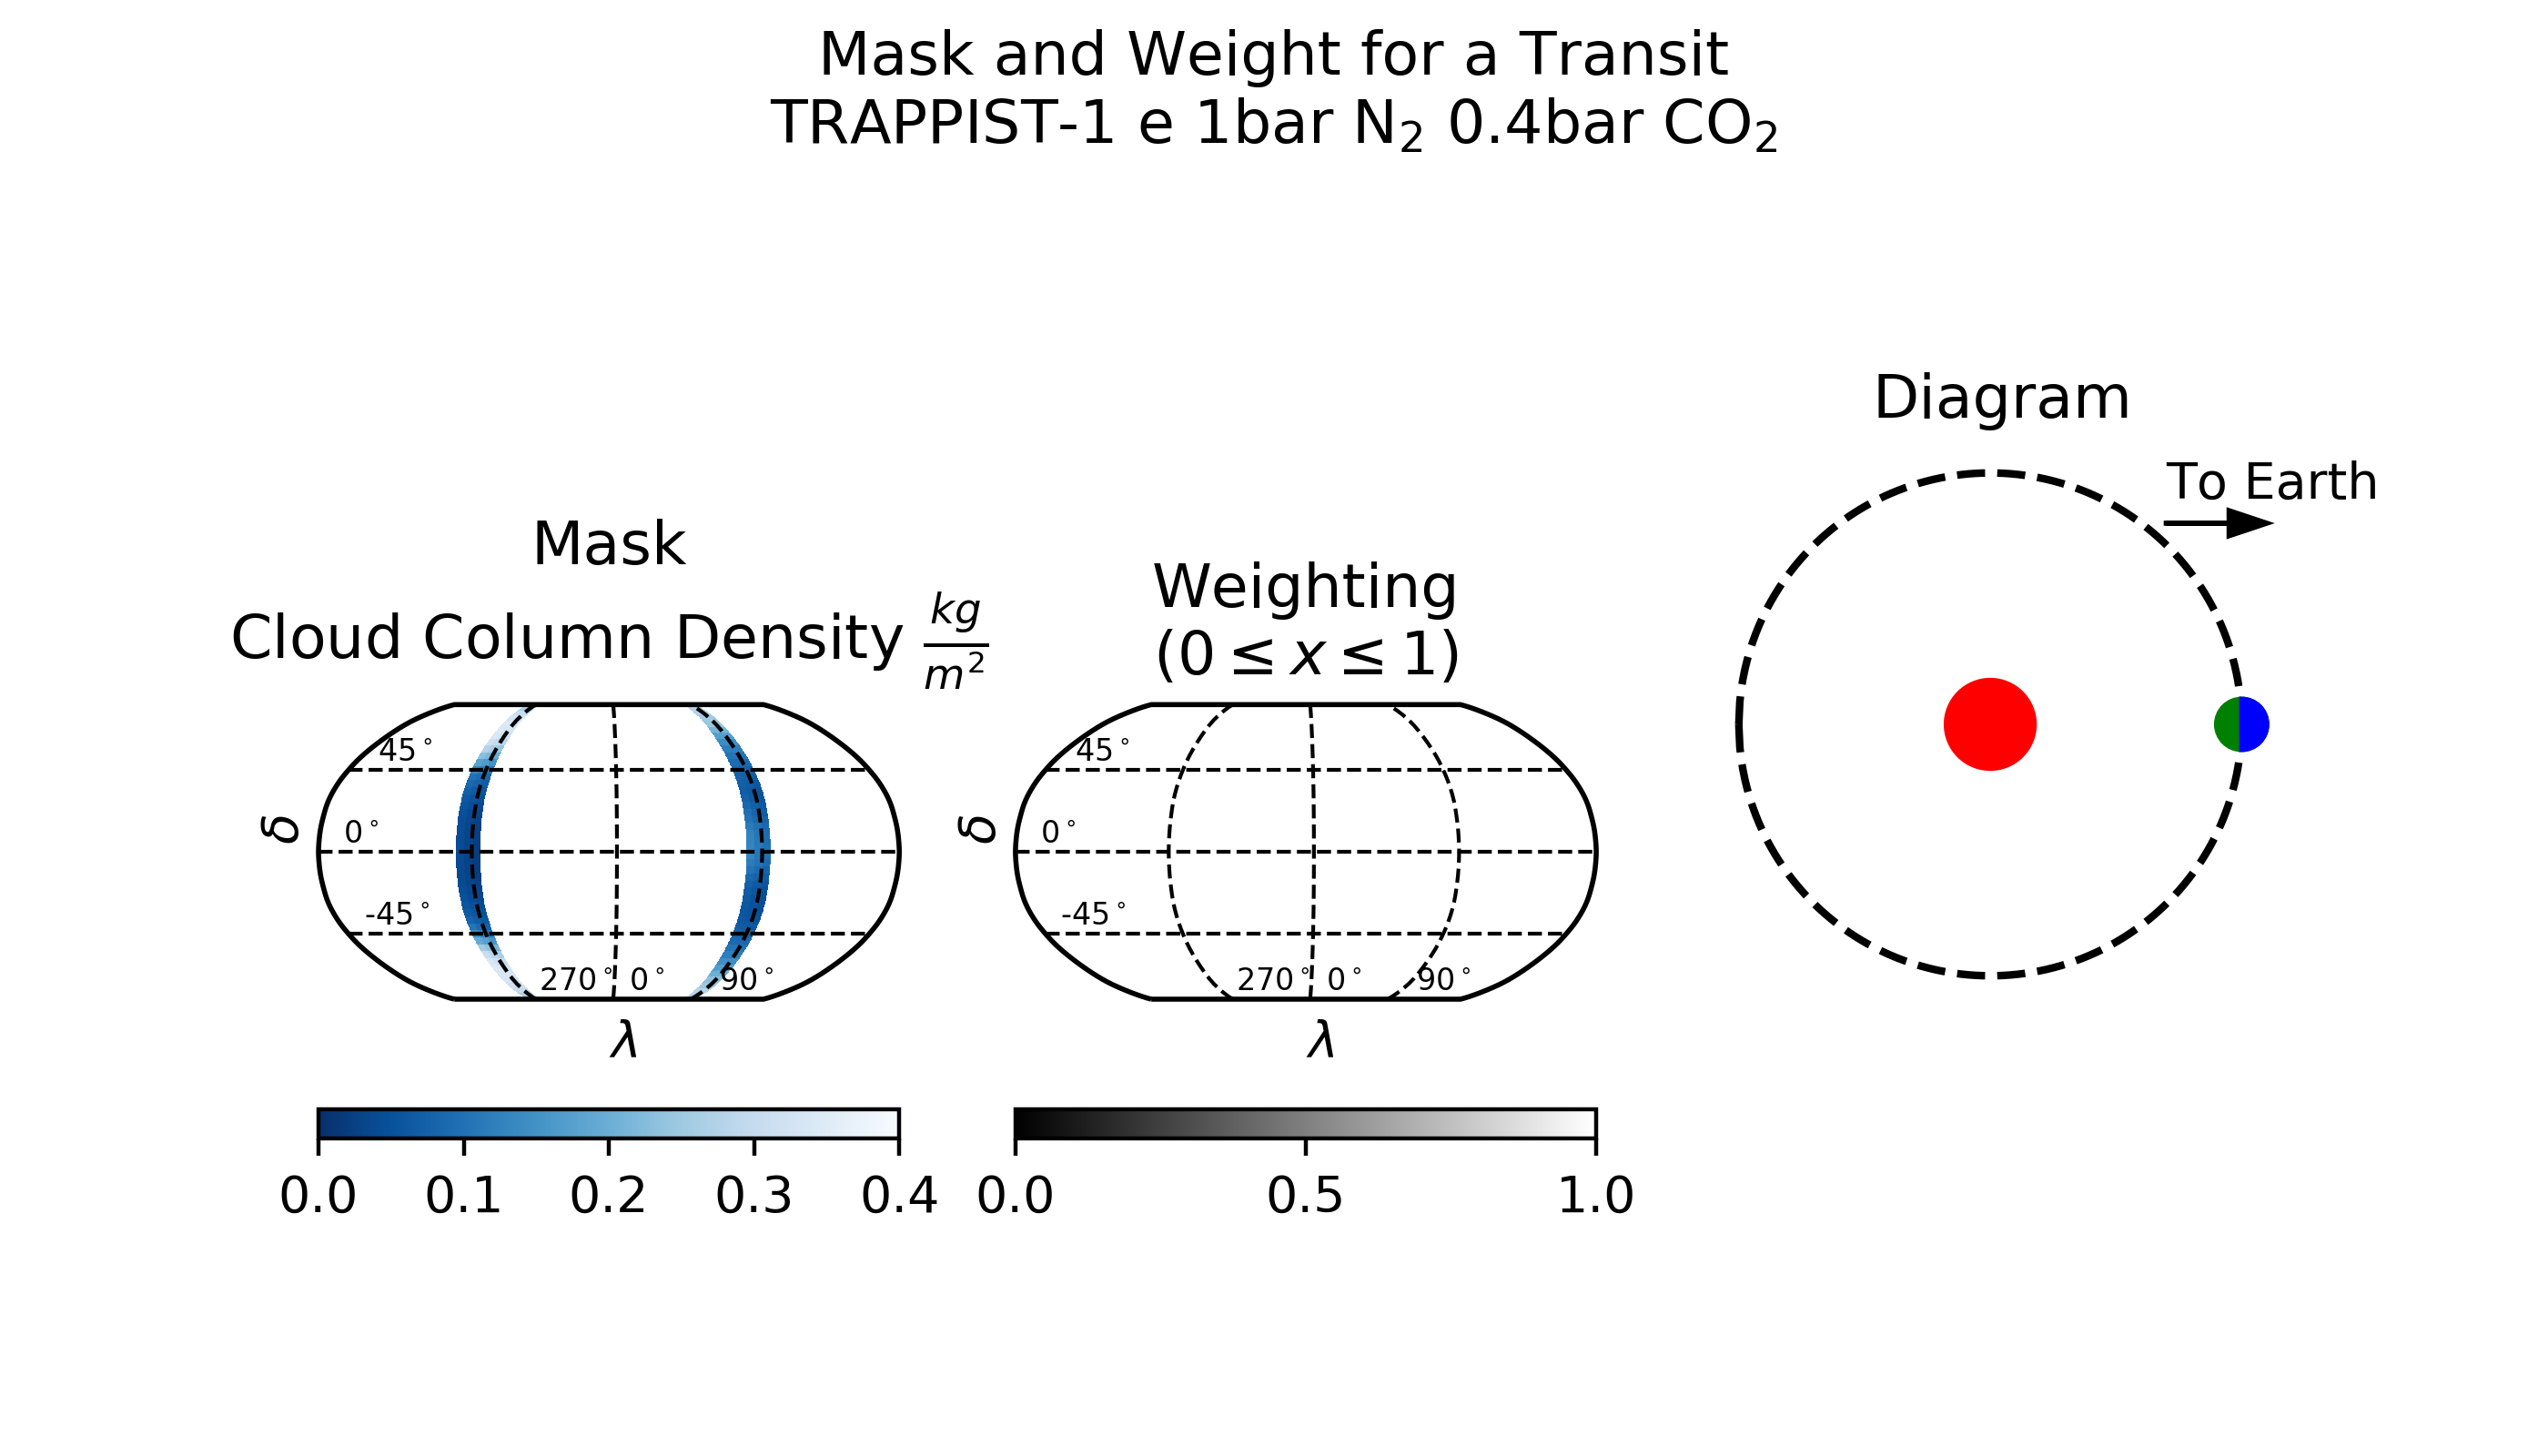
\includegraphics[width=\textwidth]{methods/transit_weights.png}
    \end{figure}
\end{frame}

\section{Transits}


\begin{frame}
    \frametitle{Infrared transit spectra has wide features, and identifying them
    is always difficult}
    \begin{figure}
        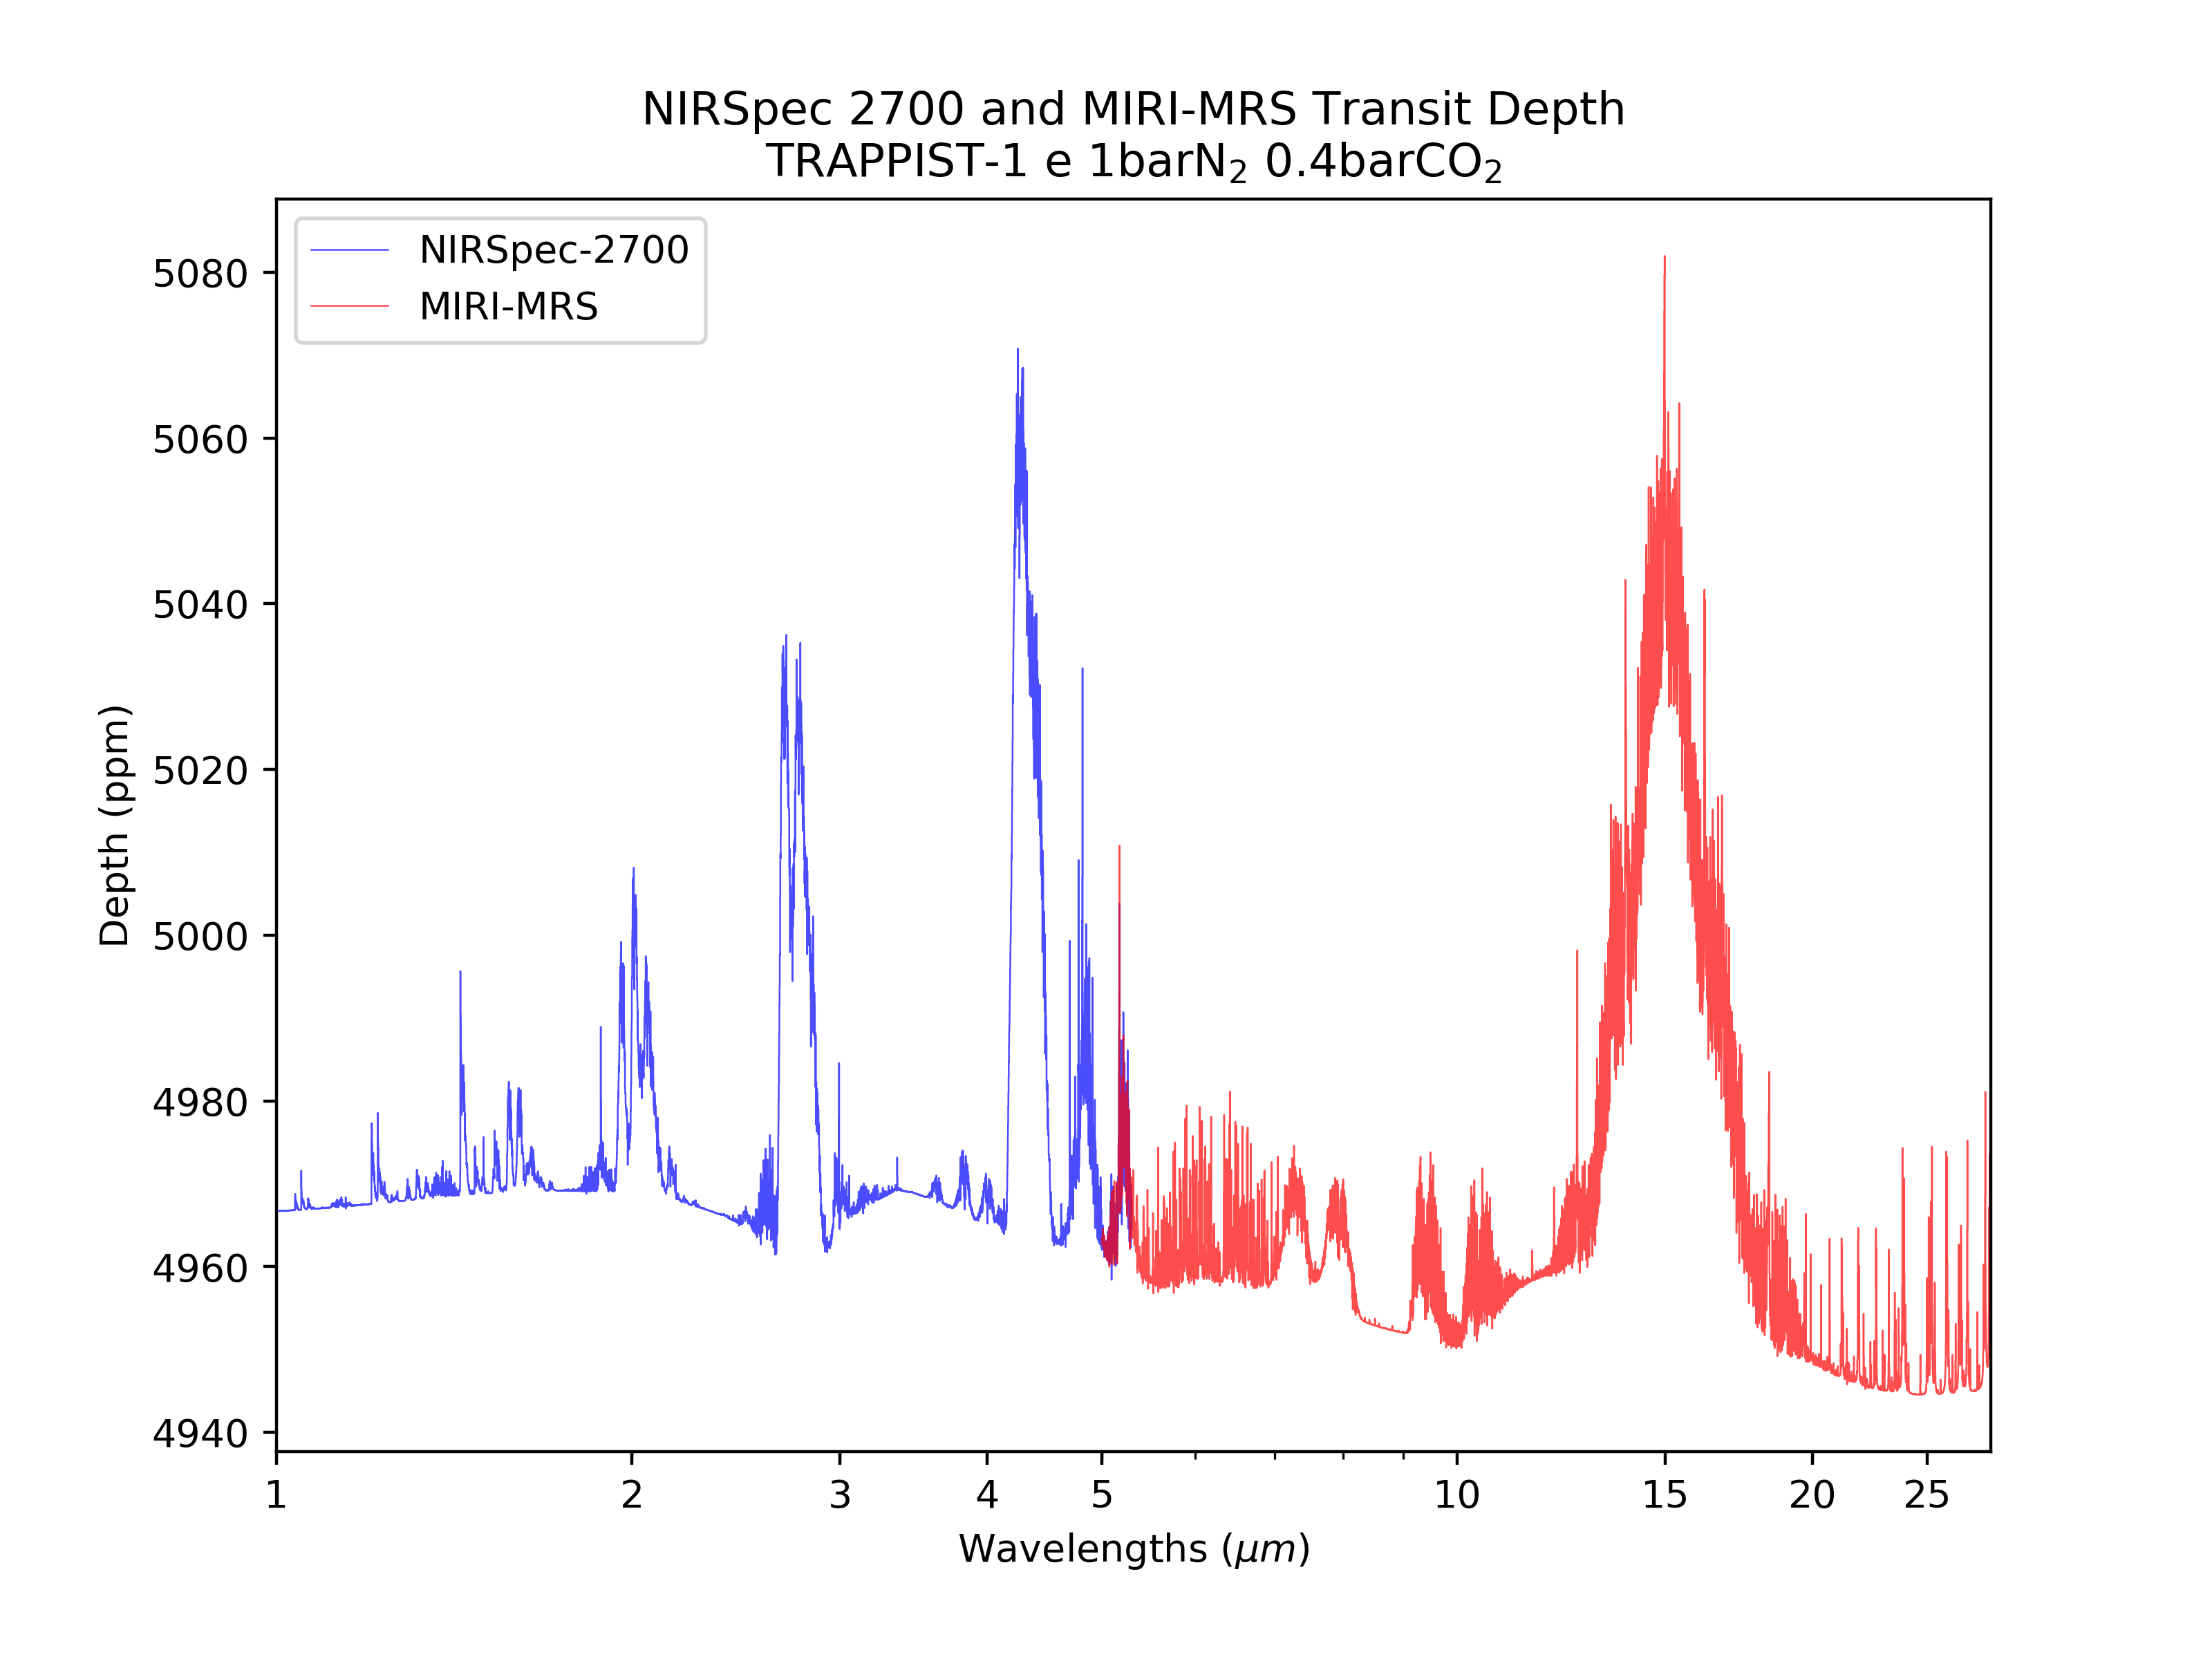
\includegraphics[height=0.8\textheight]{spectra/miri_nirspec_depth.png}
    \end{figure}
\end{frame}

\subsection{Missing species}
\begin{frame}
    \frametitle{Multiple PSG runs can determine which species are significant at
    particular wavelengths}
    \begin{figure}
        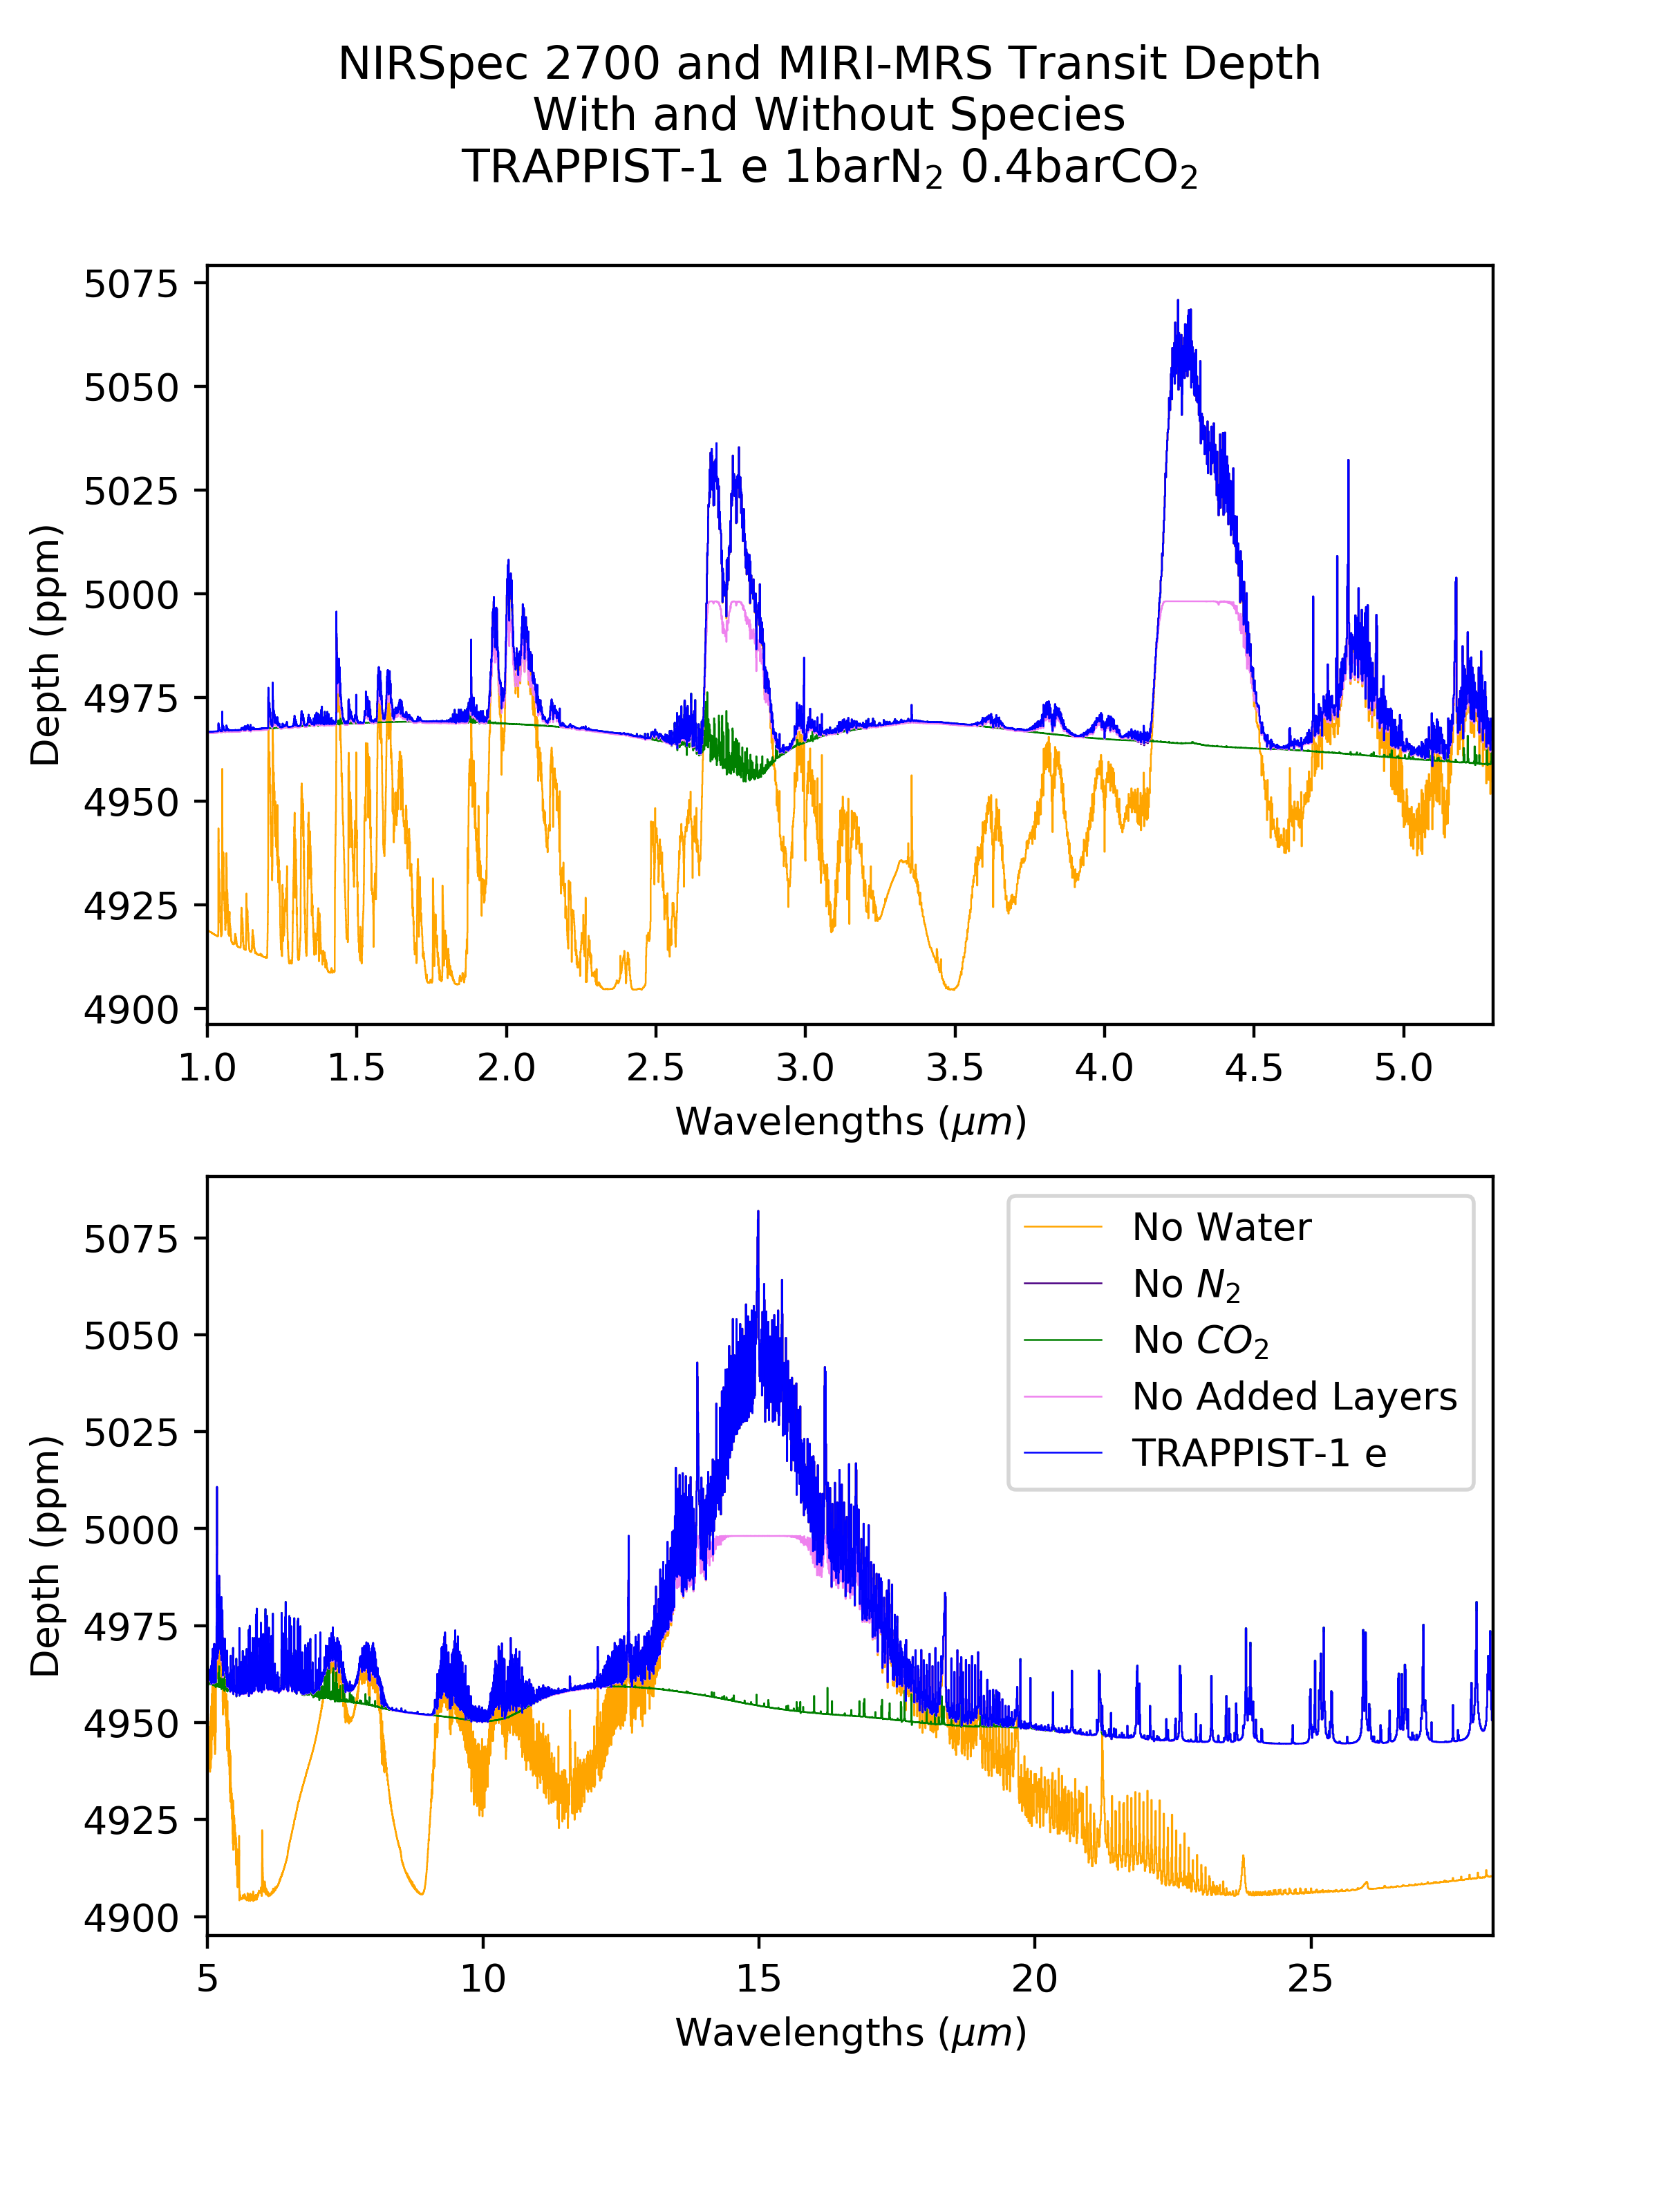
\includegraphics[height=0.95\textheight]{spectra/nirmiri_without_species.png}
    \end{figure}
\end{frame}

\subsection{Spectra across models}
\begin{frame}
    \frametitle{Transit depth depends mostly on surface temperature, not partial
    pressure}
    \begin{columns}
    \column{0.5\textwidth}
        \begin{figure}
            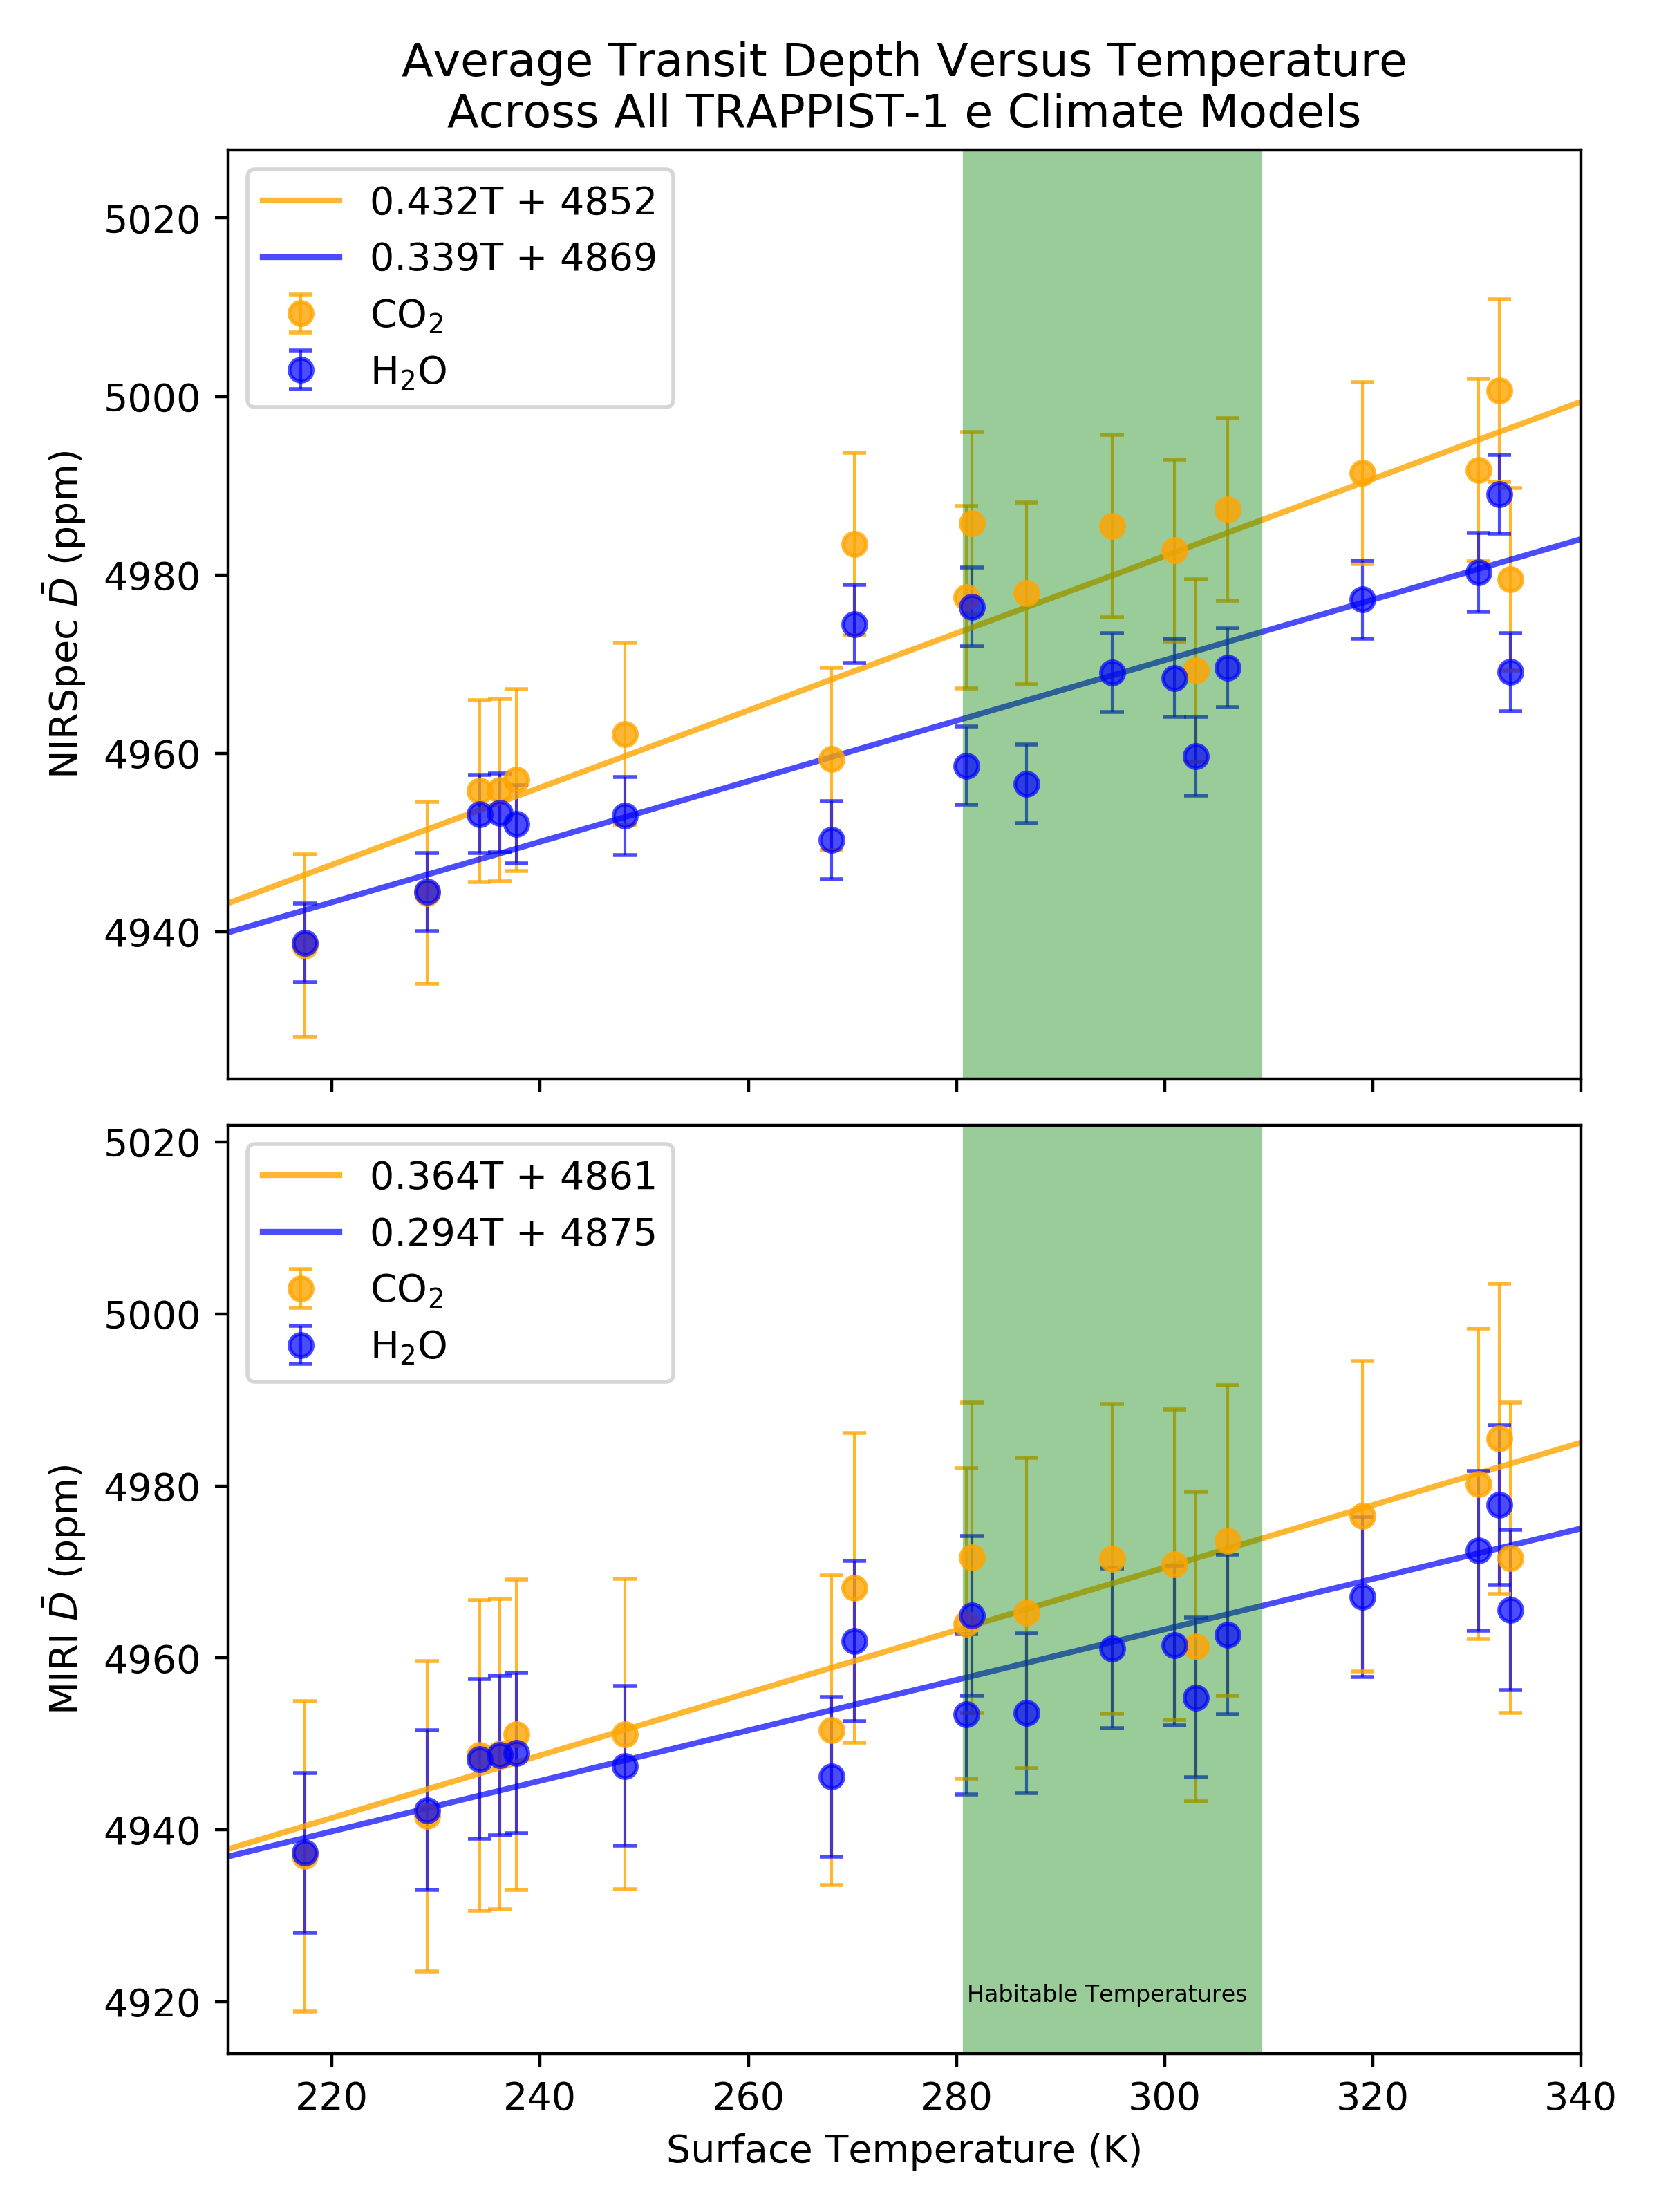
\includegraphics[width=\textwidth]{spectra/depth_from_temp.png}
        \end{figure}
    \column{0.5\textwidth}
        \begin{figure}
            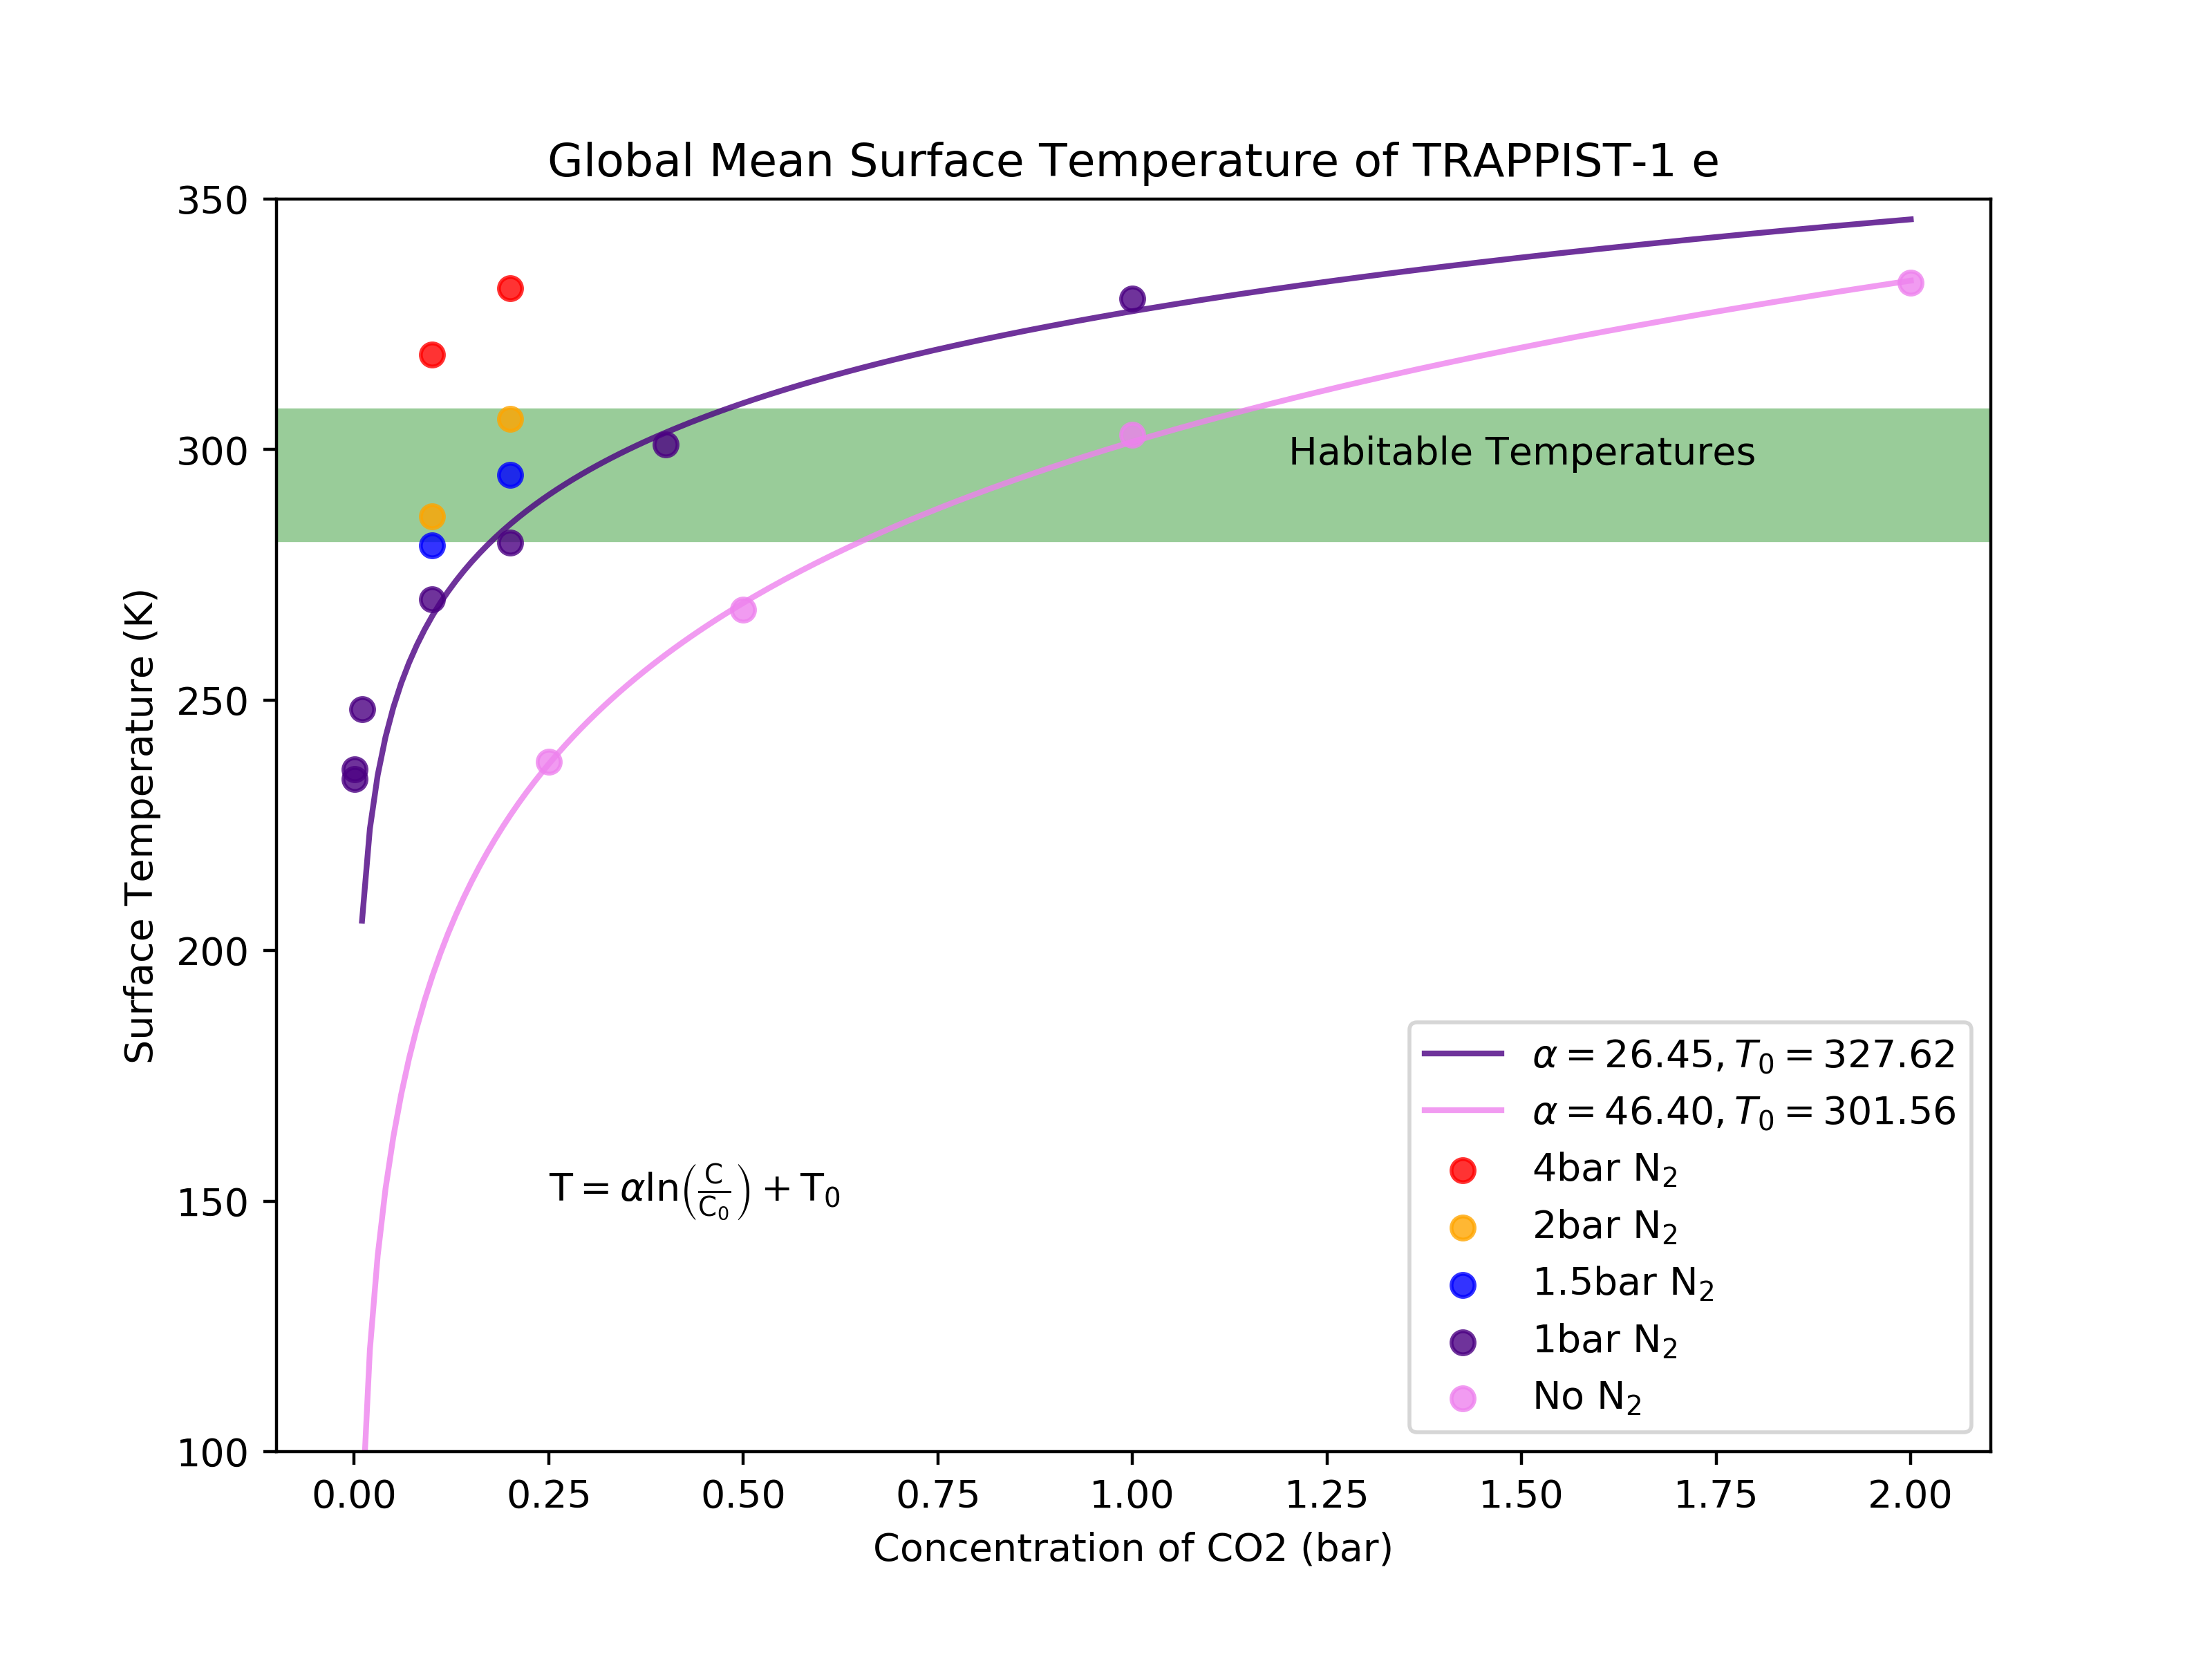
\includegraphics[width=\textwidth]{models/surfacet_co2.png}
        \end{figure}
    \end{columns}
\end{frame}

\section{Thermal Phase Curves}
\begin{frame}
    \frametitle{Like with transits, not all wavelengths will produce significant
    results for thermal phase curves}
    \begin{figure}
        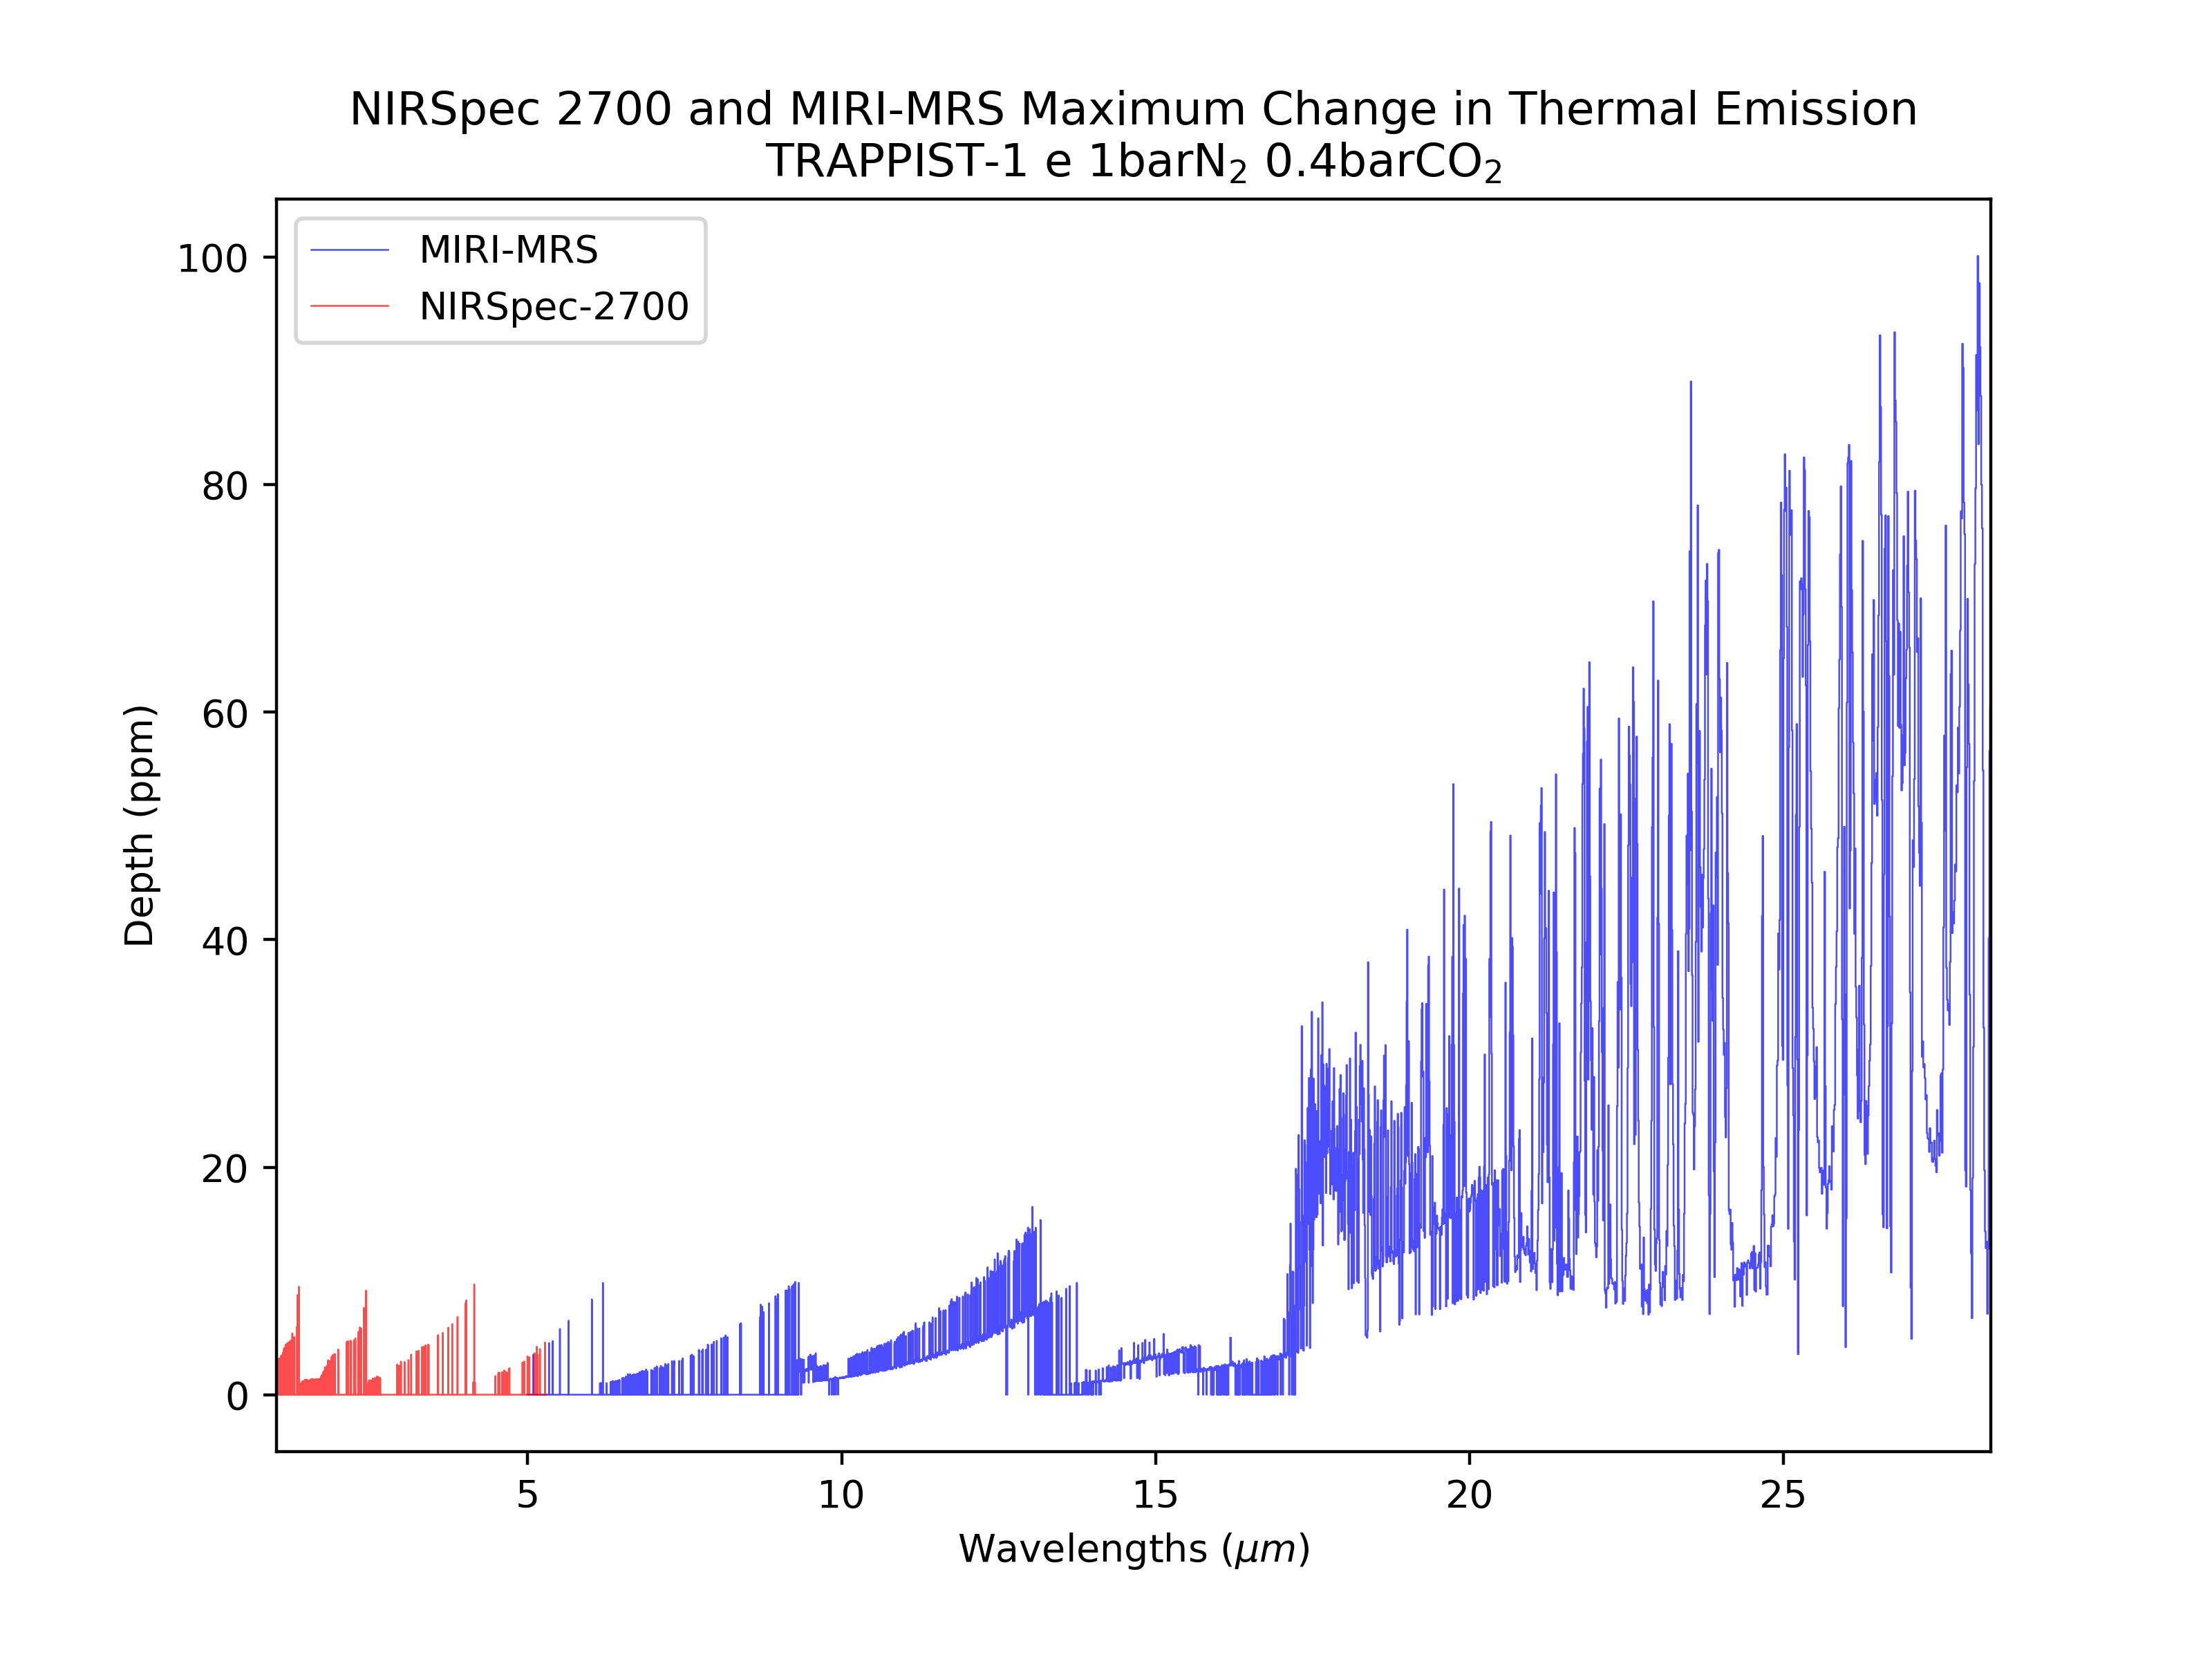
\includegraphics[height=0.9\textheight]{tpc/tpc_max_diff.png}
    \end{figure}
\end{frame}

\begin{frame}
    \frametitle{Different models produce different thermal phase curves}
    \begin{figure}
        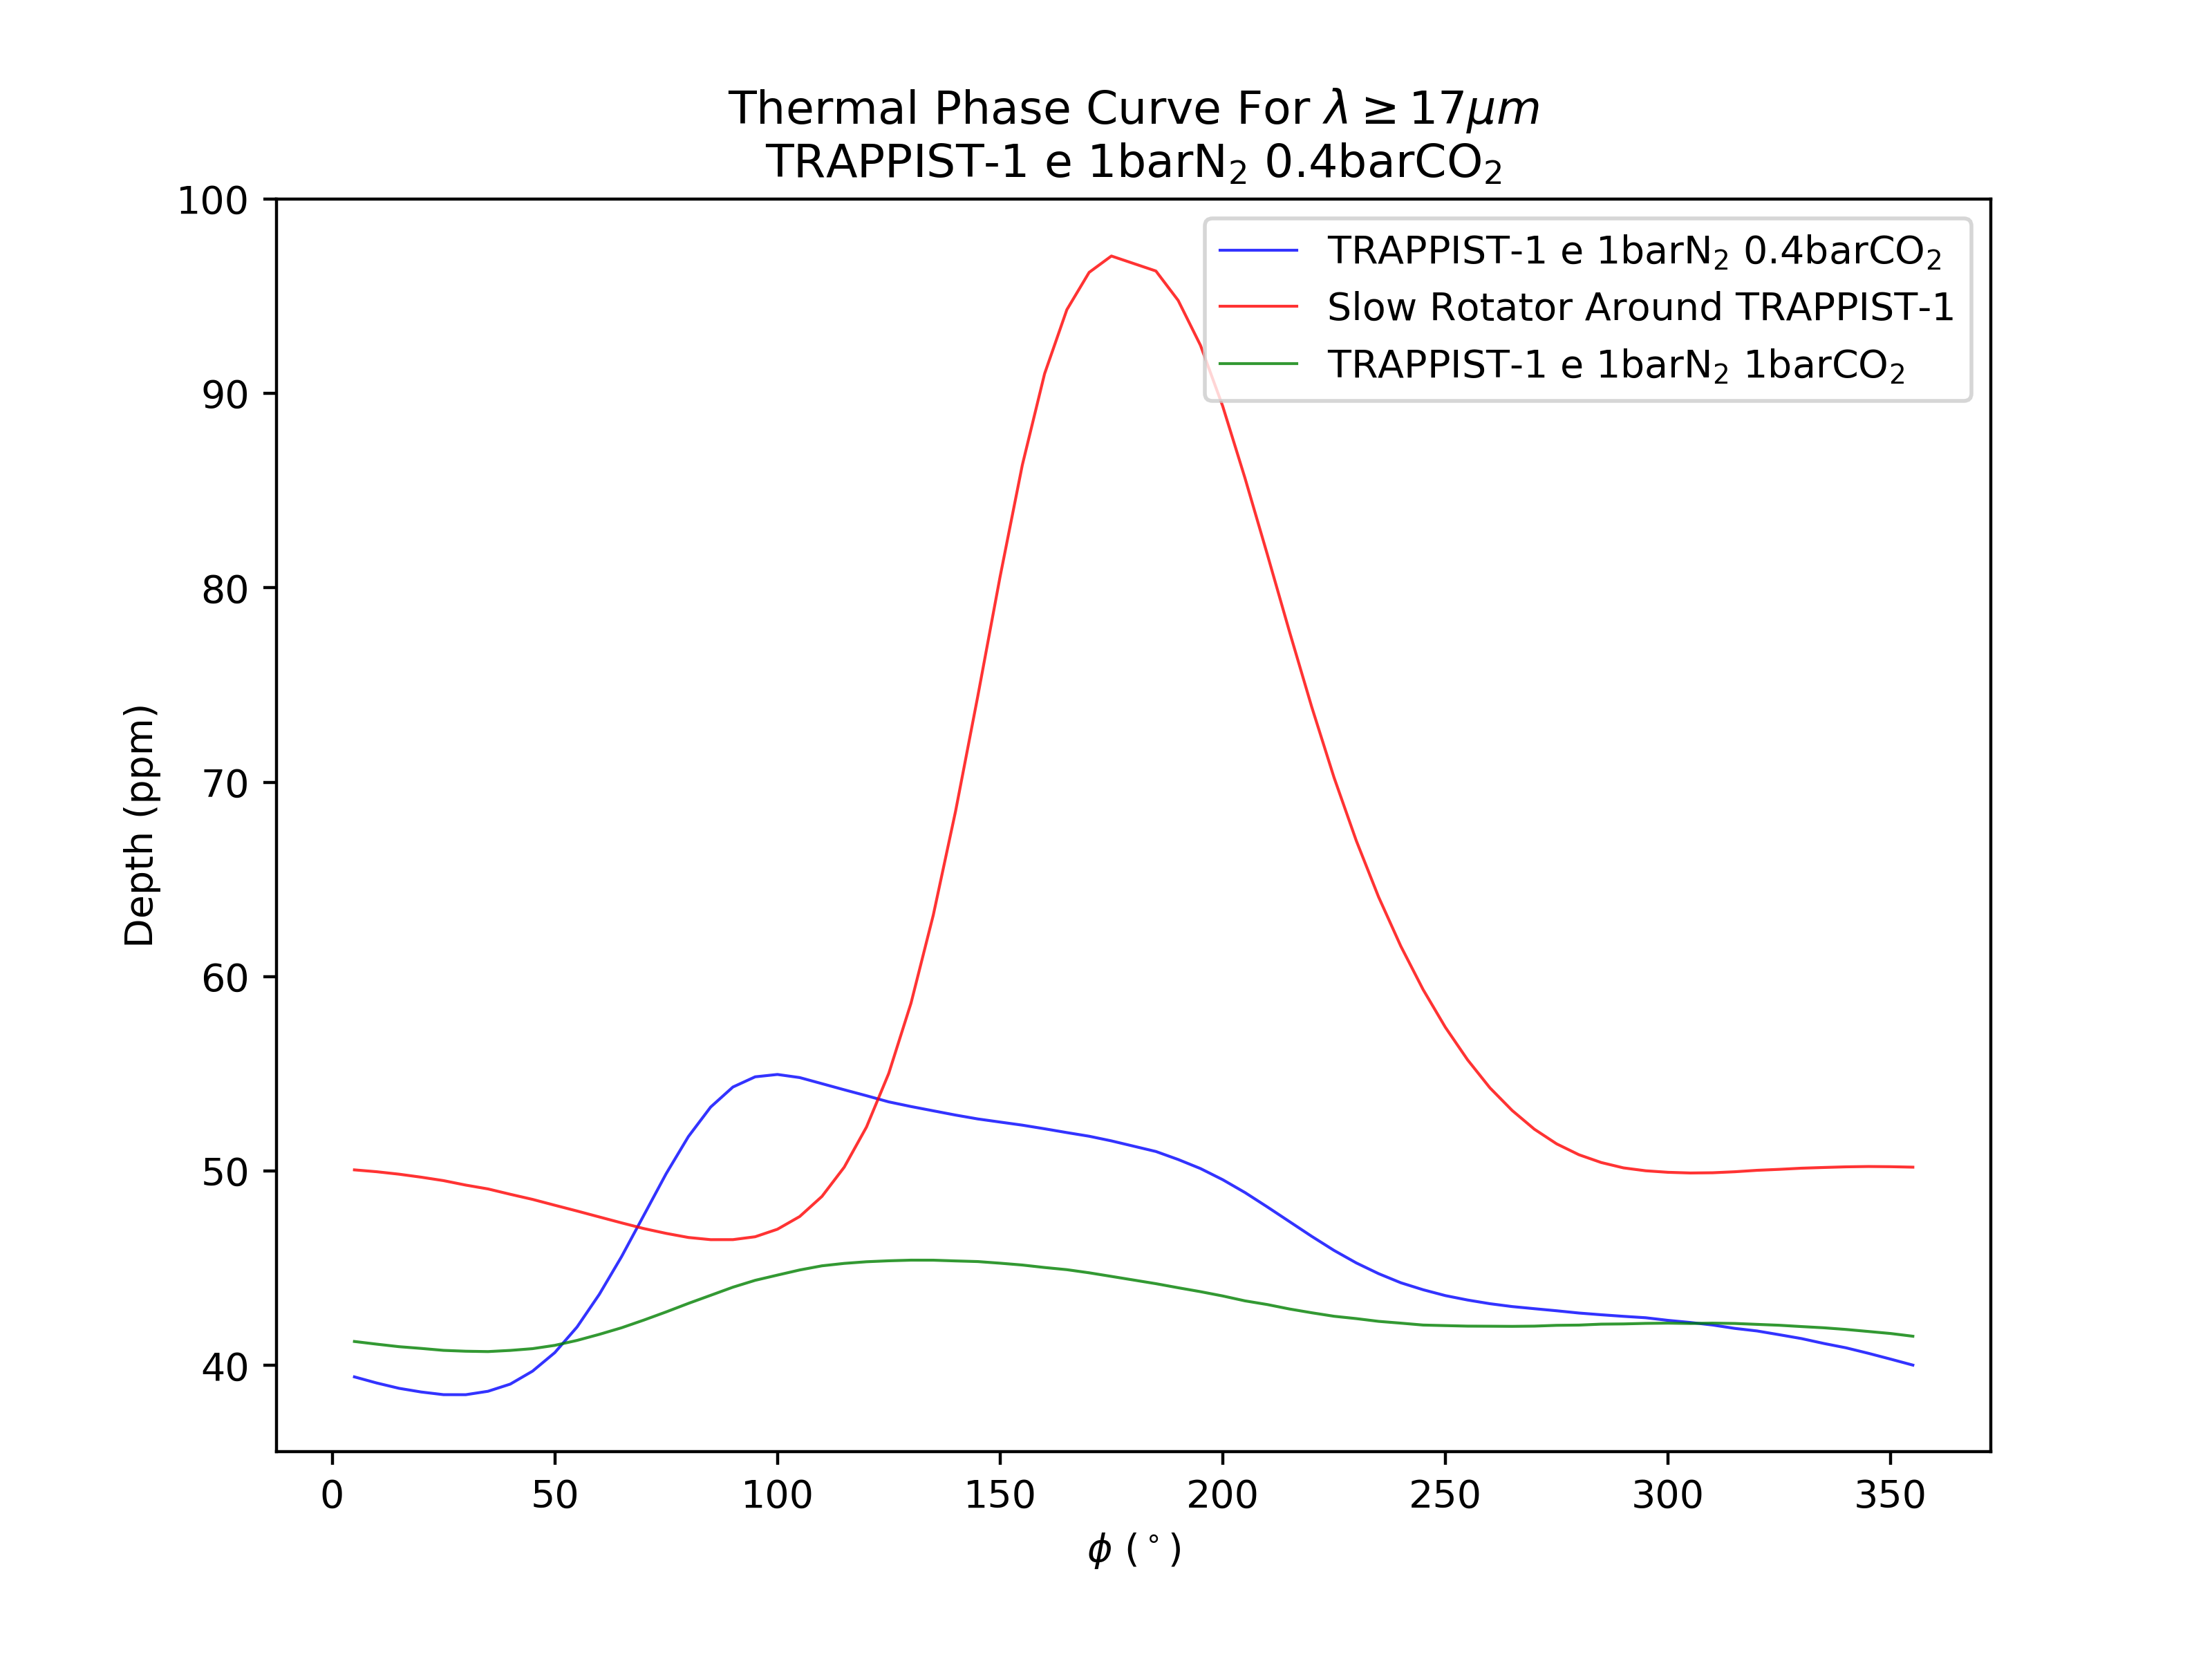
\includegraphics[height=0.9\textheight]{tpc/thermal_phase_curve.png}
    \end{figure}
\end{frame}

\section{Conclusion}
\begin{frame}
    \frametitle{Advantages and disadvantages of each method}
    \begin{columns}
    \column{0.5\textwidth}
        {\Large Transit Spectra}
        \begin{itemize}
            \item Optimal for determining species and surface temperature

            \item Requires many transits ($\sim10$) to reduce noise

            \item Actual observations are only 2-3 hours at a time

            \item Best done using spectroscopy
        \end{itemize}
    \column{0.5\textwidth}
        {\Large Thermal Phase Curves}
        \begin{itemize}
            \item Optimal for determining cloud structure and habitability

            \item Requires long observations across multiple days

            \item Requires accurate climate models to match with observations

            \item Best done using photometry
        \end{itemize}
    \end{columns}
\end{frame}

\begin{frame}
    \frametitle{References}
    \bibliographystyle{aasjournal}
    \bibliography{thesis_citations}
\end{frame}


\end{document}

